%% ----------------------------------------------------------------
%% Thesis.tex -- MAIN FILE (the one that you compile with LaTeX)
%% ---------------------------------------------------------------- 

% Set up the document
\documentclass[a4paper, 11pt, oneside]{uet_thesis}  % Use the "Thesis" style, based on the ECS Thesis style by Steve Gunn
\graphicspath{{Figures/}}  % Location of the graphics files (set up for graphics to be in PDF format)

% Include any extra LaTeX packages required
\usepackage[square, numbers, comma, sort&compress]{natbib}  % Use the "Natbib" style for the references in the Bibliography

\usepackage{verbatim}  % Needed for the "comment" environment to make LaTeX comments
\usepackage{vector}  % Allows "\bvec{}" and "\buvec{}" for "blackboard" style bold vectors in maths
\usepackage{url}

\usepackage{enumitem}
\usepackage{booktabs}
% \usepackage[margin=1in]{geometry}
\usepackage{caption}
\usepackage{graphicx}
\usepackage[utf8]{inputenc}
\usepackage{hyperref}
\usepackage{amsfonts}
\usepackage{amsmath, amssymb}
% \usepackage{geometry}
\usepackage{enumitem}
% \usepackage{titlesec}
\usepackage{tikz}
\usepackage{float}

\usepackage{listings}
\usepackage{xcolor}  % Optional: for adding colors to the code
\lstset{ 
  language=Python, 
  backgroundcolor=\color{white},   % Background color for the code block
  basicstyle=\ttfamily\small,      % Font style and size
  breaklines=true,                 % Line breaks
  frame=single,                    % Adds a frame around the code
  keywordstyle=\color{blue},       % Style for keywords
  commentstyle=\color{green},      % Style for comments
  stringstyle=\color{red},         % Style for strings
}

\hypersetup{urlcolor=blue, colorlinks=true}  % Colours hyperlinks in blue, but this can be distracting if there are many links.

% remove the unnecessary spacing before and after the headings/subheadings
\usepackage[compact]{titlesec}
\titlespacing{\section}{0pt}{*0}{*0}
\titlespacing{\subsection}{0pt}{*0}{*0}
\titlespacing{\subsubsection}{0pt}{*0}{*0}

\setlength{\parskip}{6pt}
%\setlength{\parsep}{0pt}
%\setlength{\headsep}{0pt}
%\setlength{\topskip}{0pt}

%% ----------------------------------------------------------------
\begin{document}
\frontmatter	  % Begin Roman style (i, ii, iii, iv...) page numbering

% Set up the Title Page
\title  {SMART-SBERT with SimCSE: A Robust Defense Against Catastrophic Forgetting in BERT}
%\session {2006 -- 2010}
\advisor {Dr. Irfan Ullah Chaudhry}
\authors {
Rooshan Khan  ~~~~~~~ 2021-EE-067\\
Hussnain Amjad ~~~~~ 2021-EE-063\\
Abdul Samad ~~~~~~~~~ 2021-EE-191\\ 
Areesha Noor~~~~~~~~~~ 2021-EE-103\\
}

\addresses  {\deptname \\ \univname}  % Do not change this here, instead these must be set in the "Thesis.cls" file, please look through it instead
\date       {\today}
\subject    {}
\keywords   {}

\maketitle
%% ----------------------------------------------------------------

\setstretch{1.3}  % It is better to have smaller font and larger line spacing than the other way round

% Define the page headers using the FancyHdr package and set up for one-sided printing
\fancyhead{}  % Clears all page headers and footers
\rhead{\thepage}  % Sets the right side header to show the page number
\lhead{}  % Clears the left side page header

\pagestyle{fancy}  % Finally, use the "fancy" page style to implement the FancyHdr headers


%% Select only one of the certification pages  
%\CertificationMSc{}
\CertificationBSc{}
\clearpage  % Certification ended, now start a new page


%% ----------------------------------------------------------------
% Declaration Page required for the Thesis, your institution may give you a different text to place here
\Declaration{
%\addtocontents{toc}{\vspace{1em}}  % Add a gap in the Contents, for aesthetics

We declare that the work contained in this thesis is our own, except where explicitly stated otherwise. In addition this work has not been submitted to obtain another degree or professional qualification.

\bigskip

Signed:~~ \rule[0em]{10em}{1.0pt} \\ % This prints a line for the signature 
Date:~~~~ \rule[0em]{10em}{1.0pt}  % This prints a line to write the date
}
\clearpage     % Declaration ended, now start a new page

%% ----------------------------------------------------------------

\setstretch{1.3}  % Reset the line-spacing to 1.3 for body text (if it has changed)

% The Acknowledgements page, for thanking everyone
\acknowledgements{
%\addtocontents{toc}{\vspace{1em}}  % Add a gap in the Contents, for aesthetics

We would like to express our heartfelt gratitude to our supervisor, Dr. Irfan Ullah Chaudhry, for his invaluable guidance, continuous support, and encouragement throughout the course of this project.

We are also deeply thankful to Dr. Haroon Babri for his insightful suggestions and constructive feedback, which significantly enhanced our understanding and progress.

Lastly, we extend our sincere appreciation to Mr. Asad Ullah Khan for his consistent assistance and helpful input during the course of this work.
}
\clearpage  % End of the Acknowledgements

%% ----------------------------------------------------------------

% Begin the Dedication page
\setstretch{1.3}  % Return the line spacing back to 1.3
\pagestyle{empty}  % Page style needs to be empty for this page
\dedicatory{Dedicated to our parents and teachers, whose unwavering support, guidance, and encouragement have been the foundation of our journey and success.}

\clearpage 	% End of the Dedication
%% ----------------------------------------------------------------

% Begin the Sustainable Development Goals page
\setstretch{1.3}  % Return the line spacing back to 1.3
\pagestyle{plain}  % Page style needs to be empty for this page

\addtotoc{Contribution to Sustainable Development Goals}
\vspace{0.5in}
\begin{center}
	\huge{\bf Contribution to Sustainable Development Goals} 
	\par
\end{center}

\vspace{0.5in}
We believe our thesis, \textbf{``SMART-SBERT with SimCSE: A Robust Defense Against Catastrophic Forgetting in BERT,''} makes an important contribution to the Sustainable Development Goals (SDGs) by advancing Artificial Intelligence (AI) and Natural Language Processing (NLP).

\begin{itemize}
    \item \textbf{Quality Education} \\
    Our work helps improve the reliability and flexibility of NLP models like BERT. These better models can power smarter educational tools. For example, by improving sentiment analysis, educational platforms can better understand how students feel and respond to their feedback. Similarly, enhancements in semantic textual similarity can support more accurate automated grading and personalized learning experiences. Ultimately, these advances can help improve learning outcomes and make quality education more accessible.

    \item \textbf{Industry, Innovation and Infrastructure} \\
    At the heart of our thesis is innovation in AI and NLP. We’ve developed models that reduce catastrophic forgetting while performing well on multiple tasks, including sentiment classification, paraphrase detection, and semantic textual similarity. This helps build more robust and efficient digital systems. Because our models can adapt to new tasks sequentially without growing too large, they are well-suited for real-world industrial applications. We believe these innovations can foster technological progress and economic growth by enabling smarter data processing, automation, and intelligent systems across various industries.
\end{itemize}


\clearpage	% End of the Sustainable Development Goals
%% ----------------------------------------------------------------

\pagestyle{fancy}  %The page style headers have been "empty" all this time, now use the "fancy" headers as defined before to bring them back

%% ----------------------------------------------------------------
\lhead{\emph{Contents}}  % Set the left side page header to "Contents"
\tableofcontents  % Write out the Table of Contents

%% ----------------------------------------------------------------
\lhead{\emph{List of Figures}}  % Set the left side page header to "List if Figures"
\listoffigures  % Write out the List of Figures

%% ----------------------------------------------------------------
\lhead{\emph{List of Tables}}  % Set the left side page header to "List of Tables"
\listoftables  % Write out the List of Tables

%% ----------------------------------------------------------------
\setstretch{1.5}  % Set the line spacing to 1.5, this makes the following tables easier to read
\clearpage  % Start a new page
\lhead{\emph{Abbreviations}}  % Set the left side page header to "Abbreviations"
\listofsymbols{lp{14cm}}  % Include a list of Abbreviations (a table of two columns)
{
% \textbf{Acronym} & \textbf{W}hat (it) \textbf{S}tands \textbf{F}or \\
\textbf{NLP} & \textbf{N}atural \textbf{L}anguage \textbf{P}rocessing \\
\textbf{BERT} & \textbf{B}idirectional \textbf{E}ncoder \textbf{R}epresentations from \textbf{T}ransformers \\
\textbf{SMART} & \textbf{SM}oothness-inducing \textbf{A}dversarial \textbf{R}egularization and \textbf{BR}egman p\textbf{R}oximal poin\textbf{T} op\textbf{T}imization  \\
\textbf{SBERT} & \textbf{S}entence-\textbf{BERT} \\
\textbf{SimCSE} & \textbf{Sim}ple \textbf{C}ontrastive \textbf{S}entence \textbf{E}mbeddings \\
\textbf{MLM} & \textbf{M}asked \textbf{L}anguage \textbf{M}odel \\
\textbf{NSP} & \textbf{N}ext \textbf{S}entence \textbf{P}rediction \\
\textbf{SQuAD} & \textbf{S}tanford \textbf{Q}uestion \textbf{A}nswering \textbf{D}ataset \\
\textbf{STS} & \textbf{S}emantic \textbf{T}extual \textbf{S}imilarity \\
\textbf{STS-B} & \textbf{S}emantic \textbf{T}extual \textbf{S}imilarity \textbf{B}enchmark\\
\textbf{QQP} & \textbf{Q}uora \textbf{Q}uestion \textbf{P}airs \\
\textbf{SST} & \textbf{S}tanford \textbf{S}entiment \textbf{T}reebank\\
\textbf{SNLI} & \textbf{S}tanford \textbf{N}atural \textbf{L}anguage \textbf{I}nference\\
\textbf{FFN} & \textbf{F}eed-\textbf{F}orward \textbf{N}etwork\\
\textbf{GeLU} & \textbf{G}aussian \textbf{E}rror \textbf{L}inear \textbf{U}nit\\
\textbf{ReLU} & \textbf{Re}ctified \textbf{L}inear \textbf{U}nit\\
\textbf{KL} & \textbf{K}ullback-\textbf{L}eibler\\
\textbf{VBPP} & \textbf{V}anilla \textbf{B}regman \textbf{P}roximal \textbf{P}oint\\
\textbf{MBPP} & \textbf{M}omentum \textbf{B}regman \textbf{P}roximal \textbf{P}oint\\
\textbf{SS} & \textbf{S}MART \textbf{S}BERT\\
\textbf{SSS} & \textbf{S}MART \textbf{S}BERT with \textbf{S}imCSE\\

}

%% ----------------------------------------------------------------
% The Abstract Page
\addtotoc{Abstract}  % Add the "Abstract" page entry to the Contents
\abstract{
%\addtocontents{toc}{\vspace{1em}}  % Add a gap in the Contents, for aesthetics


We aim to build a robust model based on the BERT-base architecture that performs well on three NLP tasks—sentiment classification (SST-5), paraphrase detection (QQP), and semantic textual similarity (STS-B)—by training sequentially across tasks. A core challenge in this setup is \textit{catastrophic forgetting}, where learning a new task can degrade performance on previously learned tasks due to destructive gradient updates.

To mitigate this, we implemented the \textbf{SMART algorithm}, which introduces adversarial regularization to preserve previously acquired knowledge and avoid aggressive parameter updates. This component was implemented by Rooshan Khan. Abdul Samad and Areesha contributed contrastive learning using supervised and unsupervised loss respectively. However, we used the best among these two that is supervised SimCSE loss to maximize cosine similarity between semantically similar sentence pairs and minimize it for dissimilar ones. Hussnain Amjad implemented the SBERT architecture, for task-specific classification and regression heads for QQP and STS-B, respectively.

We got two best models:
\begin{itemize}
    \item \textbf{SMART SBERT (SS)}
    \item \textbf{SMART SBERT with SimCSE (SSS)}
\end{itemize}

\textbf{SS} performed better on the SST-5 task, while \textbf{SSS} showed superior results on the STS-B task due to the SimCSE loss function being optimized for similarity learning. Both models performed equally well on paraphrase detection. Results are shown below:

\begin{table}[H]
\centering
\begin{tabular}{|l|l|c|}
\hline
\textbf{Task} & \textbf{Metric} & \textbf{Score (SS)} \\
\hline
Sentiment Classification & Accuracy & 0.537 \\
                         & F1 Score & 0.528 \\
\hline
Paraphrase Detection     & Accuracy & 0.864 \\
                         & F1 Score & 0.864 \\
\hline
Semantic Textual Similarity & Pearson Correlation & 0.819 \\
\hline
\textbf{Overall Performance} &  & \textbf{0.770} \\
\hline
\end{tabular}
\end{table}

\[
\text{Overall performance (SS)} = \frac{\left( \frac{0.819 + 1}{2} + 0.537 + 0.864 \right)}{3} = 0.770
\]

\begin{table}[H]
\centering
\begin{tabular}{|l|l|c|}
\hline
\textbf{Task} & \textbf{Metric} & \textbf{Score (SSS)} \\
\hline
Sentiment Classification & Accuracy & 0.507 \\
                         & F1 Score & 0.494 \\
\hline
Paraphrase Detection     & Accuracy & 0.864 \\
                         & F1 Score & 0.863 \\
\hline
Semantic Textual Similarity & Pearson Correlation & 0.843 \\
\hline
\textbf{Overall Performance} &  & \textbf{0.764} \\
\hline
\end{tabular}
\end{table}

\[
\text{Overall performance (SSS)} = \frac{\left( \frac{0.843 + 1}{2} + 0.507 + 0.864 \right)}{3} = 0.764
\]

Depending on task priority, either SS or SSS may be selected. Our results show that a combination of SMART regularization and contrastive learning can effectively reduce catastrophic forgetting and achieve strong performance across all three tasks in a sequential training setup.


}
\clearpage  % Abstract ended, start a new page

%% ----------------------------------------------------------------
\mainmatter	  % Begin normal, numeric (1,2,3...) page numbering
\pagestyle{fancy}  % Return the page headers back to the "fancy" style
\onehalfspacing
% Include the chapters of the thesis, as separate files
% Just uncomment the lines as you write the chapters

% Chapter 1

\chapter{Motivations and Problem Statement (Rooshan Khan)} % Write in your own chapter title
\label{Chapter1}
\lhead{Chapter 1. \emph{Motivations and Problem Statement}} % Write in your own chapter title to set the page header

Pre-trained models like BERT (Bidirectional Encoder Representations from Transformers), presented by Devlin and colleagues in their work \textit{BERT: Pre-training of Deep Bidirectional Transformers for Language Understanding}~\cite{devlin2018bert}, have transformed natural language processing by setting new benchmarks across numerous downstream tasks. However, despite its success, the BERT model is known to suffer from issues related to \textbf{robustness}—its ability to maintain consistent performance when exposed to challenging, noisy, or perturbed inputs. Furthermore, typical fine-tuning strategies often lead to large, unstable updates, making the model prone to \textbf{overfitting}, especially when training on limited data.

In our work, we aim to improve the robustness and generalizability of the BERT model. Unlike traditional approaches where separate BERT models are fine-tuned independently for each downstream task, we adopt a \textbf{sequential fine-tuning strategy} in which a single BERT model is progressively fine-tuned across multiple tasks. Specifically, the same BERT model is trained first on paraphrase detection (QQP), then on semantic textual similarity (STS-B), and finally on sentiment analysis (SST-5). This approach allows for the transfer of useful knowledge between tasks while keeping the model size compact.

We propose a robust fine-tuning framework that integrates the following components:
\begin{itemize}
    \item \textbf{Smoothness-Inducing Adversarial Regularization:} Enhances model robustness by training it to resist small perturbations in the input space.\cite{jiang2019smart}
    \item \textbf{Bregman Proximal Point Optimization:} Prevents large and unstable parameter updates during fine-tuning, ensuring smoother convergence and reducing overfitting.\cite{jiang2019smart}
    % \item \textbf{Contrastive Learning:} Optimizes sentence embeddings by encouraging semantically similar sentence pairs to be closer in the embedding space, and dissimilar pairs to be farther apart.\cite{gao2021simcse}
    \item \textbf{Contrastive Learning:} Enhances sentence representations by pulling embeddings of semantically related sentence pairs closer together, while pushing apart those of unrelated pairs within the embedding space.

\end{itemize}

We also adopt the \textbf{Siamese Sentence-BERT (SBERT)} architecture to create meaningful sentence embeddings that capture semantic similarity, enabling efficient comparison of sentence pairs.\cite{reimers2019sentence}

Our experiments use the \textbf{BERT-Base model} due to its manageable size. However, the proposed techniques can be extended to larger BERT variants, such as BERT-Large, in future work.

Table~\ref{tasks_ratings1} presents the performance of the baseline BERT model on these tasks.
\begin{table}[h]
    \centering
    \begin{tabular}{|c|c|}
        \hline
        Tasks & Accuracies(1st 2) and Pearson Correlation (last) \\ 
        \hline
        Sentiment Analysis & 0.144 \\ 
        Paraphrase Detection & 0.369 \\ 
        Semantic Textual Similarity & -0.009 \\
        \hline
    \end{tabular}
    \caption{Tasks and Ratings for simple BERT model without finetuning}
    \label{tasks_ratings1}
\end{table}

\textbf{Motivation:} Looking at Table~\ref{tasks_ratings1}, we recognized the need for fine-tuning. We wanted to investigate how fine-tuning the same model for different tasks affects its performance on those tasks—specifically, whether it improves performance on individual tasks or has the opposite effect. We explored this question using our selected tasks. Our experiments showed a slight improvement in accuracy, but it was not significant. Hence, fine-tuning alone is not sufficient. It needs to be combined with additional techniques from research papers, which we discuss in the following sections.

% \begin{table}[h]
%     \centering
%     \begin{tabular}{|c|c|}
%         \hline
%         Tasks & Accuracies(1st 2) and Pearson Correlation (last) \\ 
%         \hline
%         Semantic Textual Similarity(20 epochs) & -0.039 \\
%         Paraphrase Detection(1 epoch) & 0.766 \\
%         Sentiment Analysis(10 epochs) & 0.523 \\
%         \hline
%     \end{tabular}
%     \caption{Tasks and Ratings for multitask fine-tuned BERT model.}
%     \label{tasks_ratings2}
% \end{table}

% Hence, fine-tuning alone is not sufficient. It needs to be combined with additional techniques from research papers, which we discuss in the following sections.
% \section{Research Papers Read}
% In our research, we have studied several key papers in the field of Natural Language Processing (NLP) to gain insights into pretraining, fine-tuning strategies, and sentence embeddings. Notably, we have reviewed \textit{BERT: Pre-training of Deep Bidirectional Transformers for Language Understanding} by Devlin et al. \cite{devlin2018bert}, \textit{SimCSE: Simple Contrastive Learning of Sentence Embeddings} by Gao et al. \cite{gao2021simcse}, \textit{How to Fine-Tune BERT for Text Classification?} by Sun et al. \cite{sun2019fine}, \textit{Sentence-BERT: Sentence Embeddings using Siamese BERT-Networks} by Reimers and Gurevych \cite{reimers2019sentence}, and \textit{SMART: Robust and Efficient Fine-Tuning for Pre-trained Natural Language Models through Principled Regularized Optimization} by Jiang et al. \cite{jiang2019smart}.

% \textbf{The aim of research paper 1(\textit{SMART: Robust and Efficient Fine-Tuning for Pre-trained Natural Language Models through Principled Regularized Optimization} by Jiang et al. \cite{jiang2019smart}):}

% Aggressive fine-tuning often causes fine tuned model to overfit the training data of downstream tasks and fail to generalize to unseen data. To address this issue a new learning framework was proposed in this paper to obtain better generalization performance. The proposed framework contains:
% \begin{itemize}
%     \item Smoothness inducing adversarial regularization which effectively manages the complexity of the model. With such regularization a small perturbation to the input does not change the output of the model much.
%     \item Bregmann Proximal Point Optimization methods introduce a trust-region-type regularization at each iteration, and then update the model only within a small neighborhood of the previous iterate. Therefore, they can effectively prevent aggressive updating and stabilize the fine-tuning process.
% \end{itemize}

% \textbf{The aim of research paper 2(\textit{Sentence-BERT: Sentence Embeddings using Siamese BERT-Networks} by Reimers and Gurevych \cite{reimers2019sentence}:}

% Traditional BERT embeddings are not optimized for sentence similarity tasks. This paper introduces architecture Sentence-BERT (SBERT) that uses Siamese network to generate meaningful sentence embeddings to improve accuracy and pearson correlation coefficient for paraphrase detection and Semantic Textual Similarity tasks respectively. Cosine Similarity is used to improve accuracies of NLP tasks involving sentence pairs.
% SBERT adds a pooling operation to the output of BERT to derive a fixed sized sentence embedding. We will experiment with three pooling strategies: Using the output of the CLS-token, computing the mean of all output vectors (MEAN strategy), and computing a max-over-time of the output vectors (MAX-strategy). The default configuration is MEAN.

% \textbf{The aim of research paper 3(\textit{SimCSE: Simple Contrastive Learning of Sentence Embeddings} by Gao et al. \cite{gao2021simcse}:}

% Contrastive learning is a self-supervised learning approach where a model learns to bring similar samples closer together while pushing dissimilar samples apart in a high-dimensional space. In the context of sentence embeddings, this means that semantically similar sentences should have high cosine similarity, while unrelated sentences should have lower similarity.

% A major issue with pre-trained BERT embeddings is anisotropy, meaning that embeddings are concentrated in a narrow subspace, reducing their effectiveness. SimCSE optimizes two key properties:

% \begin{enumerate}
%     \item \textbf{Alignment}: Positive sentence pairs have high cosine similarity.
%     \item \textbf{Uniformity}: Sentence embeddings should be evenly distributed across the space.
% \end{enumerate}

% SimCSE naturally optimizes both properties through contrastive learning, improving sentence embedding quality.

\section{Proposed Approach}
We won’t be changing the architecture of BERT. This means that the first 12 layers will be the same. We will add the task specific heads for the three downstream tasks. These task specific layers will vary as we proceed with project. The three tasks are Sentiment Analysis (Classification), Paraphrase Detection (Classification), and Semantic Textual Similarity (Regression). We will take the final sentence embedding from BERT and use it as input to the task specific layers. We will be finetuning the model for each task with its dataset for a specific number of epochs. We will do this for all the three tasks. The BERT Layers will be updated regardless of the task because gradients from all tasks will backpropagate through BERT. BERT is shared for the all the tasks. The task specific heads- Sentiment Analysis (Classification head), Paraphrase Detection (Classification head), and Semantic Textual Similarity (Regression head) - will only be updated for the task for which finetuning is being done. Other task heads won't be updated. This can be understood from Figure~\ref{PM}. We know this is not enough to get good accuracies so we plan to implement three techniques to get a fine Multi-task Model. These techniques are SMART, Contrastive Learning and Siamese Sentence BERT.

\begin{figure}[ht!]
\centering
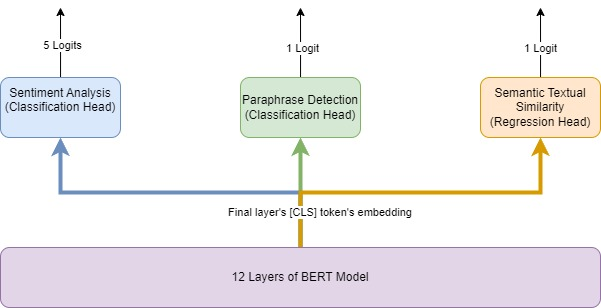
\includegraphics[width=90mm]{Figures/Proposed_Model.jpg}
\caption{Proposed Model\label{PM}}
\end{figure}
\section{Project Description}

\subsection{Data}
% \begin{itemize}
%   \item \textbf{Stanford Sentiment Treebank (SST) dataset:}
%   For the SST Dataset we have the following splits:
%   \begin{itemize}
%     \item train (8,544 examples)
%     \item dev (1,101 examples)
%     \item test (2,210 examples)
%   \end{itemize}
%   \item \textbf{Quora Dataset:}
%   For the Quora Dataset we have the following splits:
%   \begin{itemize}
%     \item train (283,010 examples)
%     \item dev (40,429 examples)
%     \item test (80,859 examples)
%   \end{itemize}
%   \item \textbf{SemEval STS Benchmark Dataset:}
%   For the  SemEval STS Benchmark Dataset we have the following splits:
%   \begin{itemize}
%     \item train (6,040 examples)
%     \item dev (863 examples)
%     \item test (1,725 examples)
%   \end{itemize}
% \end{itemize}
\begin{table}[H]
\centering
\begin{tabular}{|l|r|r|r|}
\hline
\textbf{Dataset} & \textbf{Train} & \textbf{Dev} & \textbf{Test} \\
\hline
Stanford Sentiment Treebank (SST) & 8,544 & 1,101 & 2,210 \\
\hline
Quora Question Pairs & 283,010 & 40,429 & 80,859 \\
\hline
SemEval STS Benchmark & 6,040 & 863 & 1,725 \\
\hline
SNLI & 	550,152 & Not used & Not used \\
\hline
\end{tabular}
\caption{Dataset splits used for training, validation, and testing.}
\label{tab:dataset_splits}
\end{table}

\subsection{Baseline}

We define the following baseline to estimate the upper-bound performance achievable with task-specific optimization:

\begin{itemize}
    \item \textbf{Individually fine-tuned BERT models}: Train separate BERT models, each optimized for a single task. This setup serves as a task-specific upper-bound reference using the techniques employed.
\end{itemize}


% We define the following steps to establish our experimental baselines:

% % \item \textbf{Evaluate a simple BERT model} on the three downstream tasks independently to understand baseline performance without techniques applied.

% \begin{enumerate}
%     \item \textbf{Train separately fine-tuned BERT models}, each optimized for a single task, to estimate the maximum performance achievable with the techniques used.
%     % \item \textbf{Fine-tune single BERT model} for all three tasks with task-specific output heads. We gradually apply techniques. First we use the SBERT Architecture only. Then we use SBERT Architecture and apply SMART technique as well. Then SMART SBEWRT with SimCSE. We select model with best accuracy. 
% \end{enumerate}
% % \item \textbf{Evaluate performance after integrating each advanced technique}—SMART, Contrastive Learning, and Siamese SBERT—into the multi-task setup, assessing the impact of these techniques.

\subsection{Evaluation}
We evaluate our approach on three benchmark NLP tasks:
\begin{table}[H]
    \centering
    \begin{tabular}{|c|c|}
    \hline
    \textbf{Task} & \textbf{Evaluation Metric} \\
    \hline
    \textbf{Paraphrase Detection (QQP)} & Accuracy \\
    \hline
    \textbf{Semantic Textual Similarity (STS-B)} & Pearson correlation coefficient \\
    \hline
    \textbf{Sentiment Analysis (SST-5)} & Accuracy \\
    \hline
    \end{tabular}
    \caption{Evaluation metrics for the tasks}
    \label{tasks_ratings0}
\end{table} % Introduction 

% Chapter 1

\chapter{Bidirectional Encoder Representations from Transformers: BERT (Abdul Samad)}
\label{Chapter2}
\lhead{Chapter 2. \emph{Bidirectional Encoder Representations from Transformers: BERT}} % Write in your own chapter title to set the page header

\section{Introduction}
\subsection{Bidirectional Encoder Representations from Transformers: BERT}
\subsubsection{Introduction}
Prior to BERT~\cite{devlin2018bert}, word embedding models such as Word2Vec~\cite{mikolov2013efficient} and GloVe~\cite{pennington2014glove} provided static representations for words. For instance, a word like \textit{bank} would always map to the same vector, regardless of the context in which it was used. While these models were effective for certain tasks, they struggled with capturing contextual meaning within sentences.
The advent of the Transformer architecture, with its self-attention mechanism, not only enabled parallel processing—thus utilizing the full computational power of GPUs—but also facilitated the modeling of long-range dependencies. Introduced in 2018, BERT (Bidirectional Encoder Representations from Transformers) leveraged these advancements to create deeply bidirectional contextual embeddings, revolutionizing the field of Natural Language Processing (NLP).

\section{Architecture}
BERT's architecture is based on the Transformer encoder introduced by Vaswani et al.~\cite{vaswani2017attention}, which employs stacked self-attention layers to process input sequences in parallel. Unlike decoder-based models, BERT uses only the encoder component to generate bidirectional representations.
Key architectural features include multi-head self-attention, positional embeddings, layer normalization, and residual connections. These components collectively enable BERT to capture contextual relationships between words, incorporate positional information into token representations, and stabilize training in deep networks.
BERT is primarily available in two configurations:
\begin{itemize}
    \item \textbf{BERT-base:} 12 layers, 768 hidden dimensions, 12 attention heads
    \item \textbf{BERT-large:} 24 layers, 1024 hidden dimensions, 16 attention heads
\end{itemize}
\begin{figure}[H]
\centering
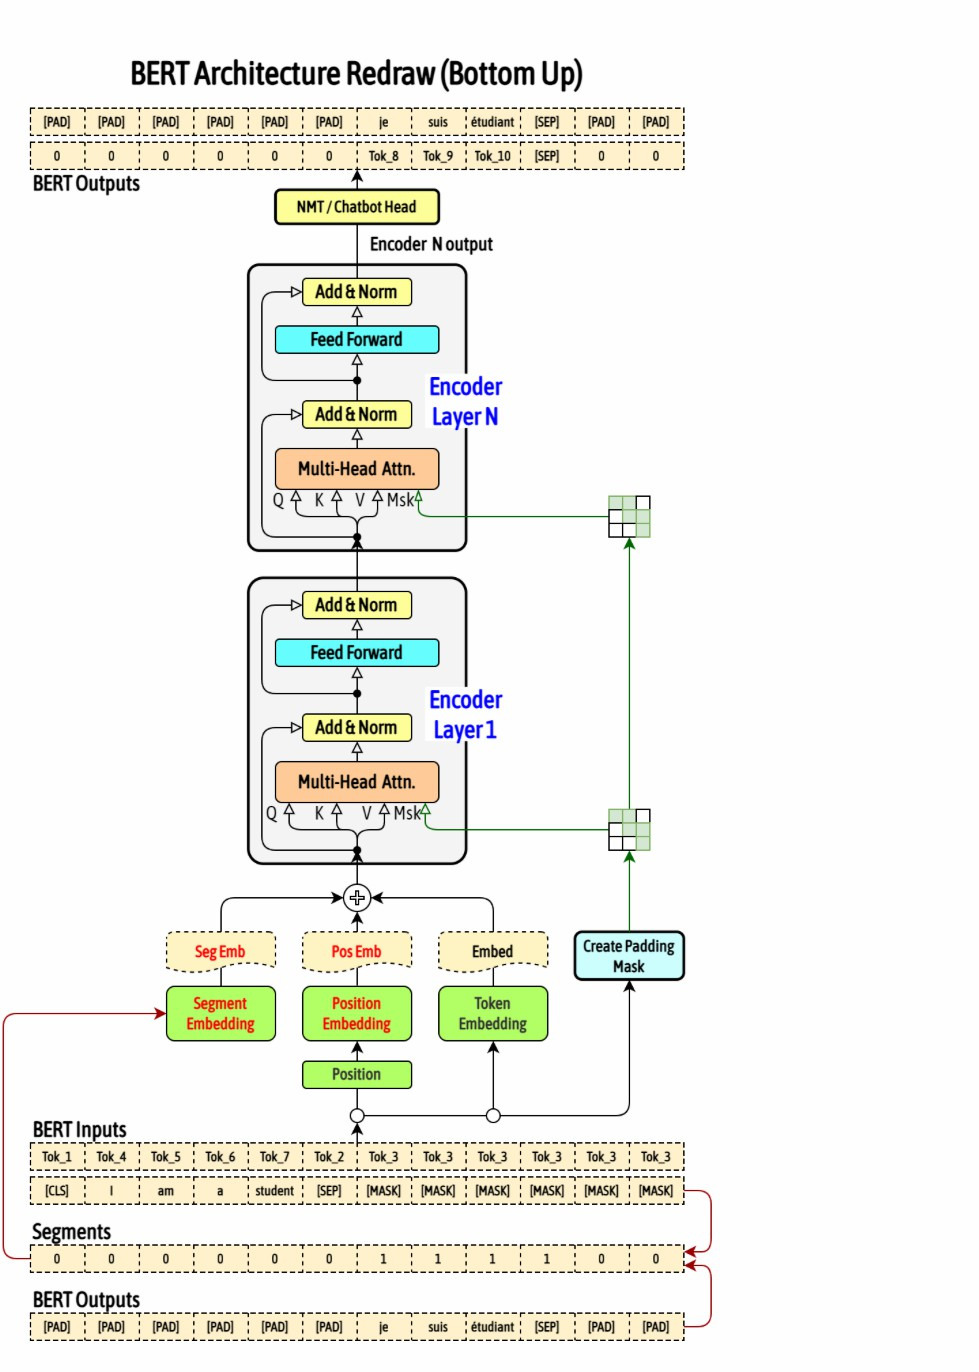
\includegraphics[width=90mm]{Figures/BERT.jpg}
\caption{BERT Architecture. Image sourced from \url{https://wikidocs.net/book/1}.\label{4}}
\end{figure}

\section{Tokenization}
BERT uses a WordPiece tokenizer to convert sentences into tokens. The main goals of tokenization are splitting words into subword units, handling out-of-vocabulary words, padding to ensure equal-length sequences, and adding special tokens \texttt{[CLS]} and \texttt{[SEP]}. As an example, the following words are converted into the following word pieces:

\begin{table}[H]
    \centering
    \begin{tabular}{|l|l|}
        \hline
        \textbf{Word} & \textbf{WordPiece Tokens} \\
        \hline
        running & [run, \#\#ing] \\
        happiness & [happi, \#\#ness] \\
        unreadable & [un, \#\#read, \#\#able] \\
        football & [foot, \#\#ball] \\
        unbelievable & [un, \#\#believ, \#\#able] \\
        \hline
    \end{tabular}
    \caption{WordPiece Tokenization}
    \label{tab:wordpiece}
\end{table}
In addition to separating each sentences into word piece token, word token that have not been seen previously will be set as \texttt{[UNK]}.

\section{Embedding Layer}
After tokenization, BERT converts each token into a high-dimensional vector using word embeddings. The embeddings are the sum of token embeddings, positional embeddings, and segmentation embeddings. The total embedding for each token is given as:
\begin{equation}\label{eqn11}
    \text{embedding}(i) = \text{token\_embedding}(i) \allowbreak + \text{position\_embedding}(i) \allowbreak + \text{segmentation\_embedding}(i)
\end{equation}

\section{Transformer Encoder Layer}
BERT is composed of 12 transformer encoder layers. Each layer integrates components such as multi-head self-attention, layer normalization, residual connections, and feed-forward networks (FFNs). The fundamental operation within the transformer is self-attention, which enables each token to consider the entire input sequence when generating its representation. In multi-head attention, the model employs \textit{n} parallel attention heads, each performing scaled dot-product attention independently. The outputs from these heads are then concatenated and passed through a linear transformation using a weight matrix \( W_o \):

\begin{equation}\label{eqn12}
    \text{MultiHead}(\text{h}) = [\text{Attention}_1(\text{h}),\dots,\text{Attention}_n(\text{h})] \text{W}_o
\end{equation}
After the computation of attention, BERT adds the original input to the attention output using a residual connection:
\begin{equation}\label{eqn13}
    \text{h}' = \text{LN}(\text{h} + \text{MultiHead}(\text{h}))
\end{equation}
\begin{equation}\label{eqn14}
    \text{SA}(h) = \text{FFN}(\text{h})
\end{equation}

where LN is layer normalization. Each encoder layer contains a feed-forward network that performs two linear transformations with a non-linear activation function applied in between:
%\begin{equation}\label{eqn15}
%    \text{FFN}(\text{h}) = \text{W}_2 \text{f} (\text{W}_1 \text{h} + \text{b}_1) + \text{b}_2
%\end{equation}
\begin{equation}\label{eqn15}
    \text{FFN}(\text{h}) = \text{W}_2 \, \text{f} (\text{W}_1 \text{h} + \text{b}_1) + \text{b}_2\footnote{FFN: Feed-Forward Network}
\end{equation}

where \textit{f(.)} is an non linearity, we use GeLU in BERT  rather than ReLU. The Gaussian Error Linear Unit (GeLU) and Rectified Linear Unit (ReLU) are both activation functions that are widely used in neural networks, but their differences in handling negative values make GeLU particularly effective in complex models like BERT  whereas ReLU, defined as ReLU(x)=max(0,x), outputs zero for all negative inputs, creating a strict boundary at zero. GeLU introduces a smooth, probabilistic transition for negative values near zero. This smoothness ensures GeLU avoids abrupt saturation, maintaining gradient flow even for inputs slightly below zero.

\section{Pre-training and Fine-tuning BERT Model}
One of the biggest challenges in language model training is to determine a prediction goal. A directional method that may restrict context learning is used by several models to predict the next word in a sequence. BERT uses two advanced methods of training to address this issue:
\begin{itemize}
    \item \textbf{Masked Language Model (MLM)}  
    The MLM task helps BERT understand words by using their surrounding context. During training, about 15\% of the words in each sentence are selected for masking:
    \begin{itemize}
        \item 80\% of these words are replaced with the special \texttt{[MASK]} token.
        \item 10\% are replaced with random words.
        \item 10\% stay the same.
    \end{itemize}
    BERT is then trained to guess the original word at each masked position using the other words in the sentence. A classifier layer on top of BERT predicts the correct word from the vocabulary. Since it only tries to guess the masked words, BERT becomes very good at understanding context in both directions.
    
    \item \textbf{Next Sentence Prediction (NSP)}  
    The NSP task helps BERT understand how sentences are related. In this task, BERT is given two sentences and must decide if the second sentence follows the first one in the original text. 
    \begin{itemize}
        \item 50\% of the time, the second sentence is correct.
        \item 50\% of the time, it is a random sentence from somewhere else.
    \end{itemize}
    To prepare the input:
    \begin{itemize}
        \item A \texttt{[CLS]} token is added at the start.
        \item A \texttt{[SEP]} token separates the two sentences.
        \item Segment embeddings mark which words belong to Sentence A or Sentence B.
        \item Positional embeddings encode the position of each token within the input sequence.

    \end{itemize}
    The output from the \texttt{[CLS]} token is passed through a small classifier that predicts whether the second sentence follows the first. A softmax function is used to give a probability.
\end{itemize}

\begin{equation}\label{eqn16}
    \text{Total Loss} = \text{NSP Loss} + \text{MLM Loss}
\end{equation}

\section{Fine-tuning for Downstream Tasks}
% BERT's flexibility allows it to be fine tuned on task specific data with minimal changes in architecture like  Text Classification which adds a classifcation layer on [CLS] token's output, Named Entity Recognition which uses token level embeddings also BERT is fine-tuned for question answering tasks, such as on the SQuAD dataset\cite{rajpurkar2016squad}, by training span prediction layers to predict the start and end positions of the answer span within a given context.
BERT's versatility enables it to be fine-tuned for various NLP tasks with minimal architectural modifications. For instance, in text classification, a classification head is added on top of the [CLS] token's representation. For named entity recognition (NER), BERT leverages token-level embeddings to make predictions. In question answering tasks like those based on the SQuAD dataset~\cite{rajpurkar2016squad}, BERT is fine-tuned by learning to identify the start and end indices of the answer span within the context.


% \textbf{What is the difference between pre-training and fine-tuning BERT?}  
% During pre-training, the model is trained on unlabeled data over different pre-training tasks. For fine-tuning, the BERT model is first initialized with the pre-trained parameters, and all of the parameters are fine-tuned using labeled data from the downstream tasks.

\textbf{What is the difference between pre-training and fine-tuning BERT?} \\
Pre-training involves training the model on large-scale unlabeled text using specific self-supervised objectives. In contrast, fine-tuning adapts the pre-trained BERT model to a specific task by updating all of its parameters using labeled data relevant to that task.
 % What to Write 

\chapter{Theoretical Background}
\label{Chapter3}
\lhead{Chapter 3. \emph{Theoretical Background}} % Write in your own chapter title to set the page header
In our research, we have studied several key papers in the field of Natural Language Processing (NLP) to gain insights into pretraining, fine-tuning strategies, and sentence embeddings. The techniques that we will discuss in this chapter have been taken from some important research papers.
\section{SMART: Smoothness Inducing Adversarial Regularization and Bregman Proximal Point Optimization: Rooshan Khan}
\label{sec:SMART_theory}
This framework was introduced in the research paper \textit{SMART: Robust and Efficient Fine-Tuning for Pre-trained Natural Language Models through Principled Regularized Optimization} by Jiang et al. \cite{jiang2019smart}
Aggressive fine-tuning often causes the model to overfit the training data of downstream tasks, resulting in poor generalization to unseen data. To tackle this problem, the authors introduced a novel learning framework aimed at improving generalization performance.

\subsection{Framework Overview}

The proposed framework consists of two fundamental techniques to enhance the fine-tuning process of pre-trained language models:

\begin{enumerate}
  \item \textbf{Smoothness-Inducing Adversarial Regularization:} \\[0.5em]
  This technique enforces local smoothness by penalizing the model's sensitivity to small input perturbations. Specifically, it identifies the worst-case perturbation within an $\epsilon$-ball around each input. First, for each sample \( x_i \), we find a nearby perturbed input \( \tilde{x}_i \) that maximizes the smoothness loss. Then, we minimize the combined task and smoothness loss over model parameters \( \theta \).  A symmetrized Kullback-Leibler divergence is applied for classification tasks, while a squared loss is used for regression. This regularization effectively controls the model complexity and mitigates overfitting. The mathematics of this technique can be understood from the equations given below. We solve the following optimization for fine-tuning.
    \[
    \min_{\theta} \mathcal{F}(\theta) = \mathcal{L}(\theta) + \lambda_s \mathcal{R}_s(\theta),
    \]
    where $\mathcal{L}(\theta)$ represents the loss function which is defined as

    \[
    \mathcal{L}(\theta) = \frac{1}{n} \sum_{i=1}^{n} \ell(f(x_i; \theta), y_i),
    \]

    and $\ell(\cdot, \cdot)$ denotes the task-specific loss function (We used Binary Cross Entropy loss function for Paraphrase Detection, MSE loss function for STS, and Cross Entropy loss function for Sentiment Analysis), $\lambda_s > 0$ is a tuning parameter, and $\mathcal{R}_s(\theta)$ is the Smoothness-Inducing Adversarial Regularizer. Here we define $\mathcal{R}_s(\theta)$ as

    \[
    \mathcal{R}_s(\theta) = \frac{1}{n} \sum_{i=1}^{n} \max_{\|\tilde{x}_i - x_i\|_p \leq \epsilon} \ell_s(f(\tilde{x}_i; \theta), f(x_i; \theta)),
    \]

    where $\epsilon > 0$ is a tuning parameter. Note that for classification tasks, $f(\cdot; \theta)$ outputs a probability simplex\footnote{For \( n \) possible outcomes, a point in the probability simplex is a vector \( \mathbf{p} = (p_1, p_2, \dots, p_n) \), where \( p_i \geq 0 \) for all \( i \), and \( \sum_{i=1}^{n} p_i = 1 \).} and $\ell_s$ is chosen as the symmetrized KL-divergence, i.e.,

    \[
    \ell_s(P, Q) = \mathcal{D}_{\mathrm{KL}}(P \| Q) + \mathcal{D}_{\mathrm{KL}}(Q \| P);
    \]
    KL Divergence has the following formula:
    \[
    D_{\mathrm{KL}}(P \parallel Q) = \sum_{x \in \mathcal{X}} P(x) \log \left( \frac{P(x)}{Q(x)} \right)
    \]
    For regression tasks, $f(\cdot; \theta)$ outputs a scalar and $\ell_s$ is chosen as the squared loss, i.e.,
    \[
    \ell_s(p, q) = (p - q)^2.
    \]

  \item \textbf{Bregman Proximal Point Optimization:} \\[0.5em]
  To stabilize fine-tuning, this method adds a penalty based on a Bregman divergence that constrains parameter updates. It ensures that each update remains close to the previous parameters, thereby preventing excessively aggressive changes. A momentum variant further accelerates convergence and enhances stability.
  The equations related to this technique are given below. At the (t+1)-th iteration, the Vanilla Bregman Proximal Point (VBPP) method takes
    \[
    \theta_{t+1} = \arg\min_{\theta} \mathcal{F}(\theta) + \mu D_{\mathrm{Breg}}(\theta, \theta_t)
    \]
    where $\mu>0$ and the Bregman Divergence is given by
    \[
    D_{\mathrm{Breg}}(\theta, \theta_t) = \frac{1}{n} \sum_{i=1}^n \ell(f(\theta; x_i), f(\theta_t; x_i))
    \]
    In our implementation we have acceleration by momemtum as well so our parameters get updated like this:
    \[
    \theta_{t+1} = \arg\min_{\theta} \mathcal{F}(\theta) + \mu D_{\mathrm{Breg}}(\theta, \tilde{\theta}_t)
    \]
    where
    \[
    \tilde{\theta}_t = (1 - \beta) \theta_t + \beta \theta_{t-1}
    \]
    is the exponential moving average and $\beta \in (0, 1)$ is the momentum parameter. This is  the momentum Bregman proximal point (MBPP)
    method.

\subsection{Implementation of SMART}

We implemented the SMART algorithm on all three tasks. We observed improvements in the accuracies of all the tasks (Sentiment Analysis, Semantic Textual Similarity, and Paraphrase Detection). We also observed that the maximum accuracy is now achieved in fewer epochs. However, the drawbacks are that the time required to train each epoch has increased by 4 to 5 times compared to training without SMART, and additional memory is required. Specifically, for the Paraphrase Detection task, each epoch now takes approximately 5 hours with SMART, compared to 50 minutes without SMART.

\end{enumerate}
\section{Mathematical Foundations and Intuition Behind Supervised SimCSE Contrastive Loss: Abdul Samad}
\subsection{Introduction}
SimCSE (Simple Contrastive Learning of Sentence Embeddings) is a powerful technique for learning sentence representations that capture semantic meaning. This technique was introduced in the reserach paper \textit{SimCSE: Simple Contrastive Learning of Sentence Embeddings} by Gao et al.~\cite{gao2021simcse}. This document explains in depth the mathematics and intuition behind the Supervised SimCSE approach and its adaptation to paraphrase detection, especially in the context of the SNLI dataset. The goal is to enable anyone with basic machine learning understanding to grasp the core concepts.

\subsection{Why Contrastive Learning?}

In traditional classification, we teach models to map inputs to fixed class labels. In contrastive learning, we teach models to understand relationships between inputs, especially:
\begin{itemize}
    \item Which examples should be close (positive pairs)
    \item Which examples should be far apart (negative pairs)
\end{itemize}

We do this by pulling similar sentence embeddings together and pushing dissimilar ones apart. The result is a semantic embedding space where cosine similarity reflects actual meaning.

\subsection{Sentence Embeddings and Similarity}

Given a sentence, BERT produces a high-dimensional vector (embedding). To compare two sentences:
\begin{enumerate}
    \item Convert both into vectors (via BERT and pooling)
    \item Normalize the vectors
    \item Measure cosine similarity:
\end{enumerate}

\[
\text{sim}(\mathbf{u}, \mathbf{v}) = \frac{\mathbf{u}^\top \mathbf{v}}{\|\mathbf{u}\| \cdot \|\mathbf{v}\|}
\]

If vectors are unit-normalized:

\[
\text{sim}(\mathbf{u}, \mathbf{v}) = \mathbf{u}^\top \mathbf{v}
\]

\subsection{Supervised SimCSE Using SNLI Triplets}

\subsubsection{Dataset Structure}

Each training example is a triplet:
\begin{itemize}
    \item Anchor ($a$): Premise
    \item Positive ($p$): Hypothesis with entailment
    \item Negative ($n$): Hypothesis with contradiction
\end{itemize}

\subsubsection{Goal}

We want:
\begin{itemize}
    \item The similarity between $a$ and $p$ to be high
    \item The similarity between $a$ and $n$ to be low
\end{itemize}

\subsubsection{Mathematical Loss Derivation}

Let:
\begin{itemize}
    \item $\mathbf{a}_i$: embedding of anchor
    \item $\mathbf{p}_i$: embedding of positive
    \item $\mathbf{n}_i$: embedding of negative
\end{itemize}

All embeddings are L2-normalized:

\[
s^+_i = \mathbf{a}_i^\top \mathbf{p}_i, \quad s^-_i = \mathbf{a}_i^\top \mathbf{n}_i
\]

Convert these into probabilities using softmax with temperature $\tau$:

\[
P_i = \frac{\exp(s^+_i / \tau)}{\exp(s^+_i / \tau) + \exp(s^-_i / \tau)}
\]

The contrastive loss per instance:

\[
\mathcal{L}_i = -\log(P_i)
\]

Overall loss per batch:

\[
\mathcal{L} = \frac{1}{N} \sum_{i=1}^{N} \mathcal{L}_i
\]

% \subsection{Contrastive Loss for Paraphrase Detection}

% \subsubsection{Problem Setup}

% Given labeled sentence pairs (e.g., Quora):
% \begin{itemize}
%     \item Each pair $(x_i, y_i)$ has label $l_i \in \{0, 1\}$
%     \item If $l_i = 1$, the pair is a paraphrase
%     \item If $l_i = 0$, it is not
% \end{itemize}

% \subsubsection{Similarity Matrix}

% Let:
% \begin{itemize}
%     \item $\mathbf{u}_i$: embedding of $x_i$
%     \item $\mathbf{v}_i$: embedding of $y_i$
% \end{itemize}

% Define similarity matrix $S \in \mathbb{R}^{N \times N}$:

% \[
% S_{ij} = \mathbf{u}_i^\top \mathbf{v}_j
% \]

% \subsubsection{Loss}

% Focus on $l_i = 1$ only:

% \[
% \mathcal{L}_i = -\log\left(\frac{\exp(S_{ii}/\tau)}{\sum_{j=1}^{N} \exp(S_{ij}/\tau)}\right)
% \]

% Total loss:

% \[
% \mathcal{L} = \frac{1}{\sum_i l_i} \sum_{i=1}^{N} l_i \cdot \mathcal{L}_i
% \]

\subsection{Temperature Parameter (\texorpdfstring{$\tau$}{τ})}

The temperature $\tau$ controls the sharpness of separation:
\begin{itemize}
    \item Small $\tau$: encourages hard separation, but may overfit
    \item Large $\tau$: softer distinction, but may underfit
\end{itemize}

Typical value: $\tau = 0.05$

\subsection{Key Takeaways}

\begin{itemize}
    \item SimCSE learns semantic sentence embeddings through contrastive learning.
    \item Cosine similarity and softmax are central to the formulation.
    \item SNLI provides well-structured triplets for training.
    % \item Quora provides paraphrase-labeled pairs useful for supervised contrastive learning.
\end{itemize}
% ---------------- SBERT SECTION (UPDATED) ----------------
\section{Implementation of Sentence-BERT architecture for Semantic Textual Similarity and Paraphrase Detection: Hussnain Amjad}
The SBERT architecture was introduced in the research paper \textit{Sentence-BERT: Sentence Embeddings using Siamese BERT-Networks} by Reimers and Gurevych~\cite{reimers2019sentence}.

\subsection{Background and Motivation}
BERT provides deep contextual language representations but lacks the capacity to generate good sentence embeddings that can be efficiently compared. Sentence-BERT (SBERT) overcomes this limitation by employing a Siamese architecture that produces meaningful sentence vectors, enabling direct comparison through distance-based metrics. In our project, SBERT was implemented and fine-tuned for two tasks: Semantic Textual Similarity (STS) and Paraphrase Detection.

\subsection{Architecture and Embedding Strategy}
Each sentence is independently passed through a shared BERT encoder. Token embeddings from the final hidden layer are then aggregated using \textbf{MEAN pooling} to form fixed-length sentence vectors. Padding tokens are excluded using an attention mask. The resulting sentence embeddings are denoted by $u$ and $v$.

\subsection{Paraphrase Detection (Classification Task)}

\textbf{Objective:} Given a pair of sentences, determine whether they are paraphrases. This is a binary classification problem.

\textbf{Embedding Interaction:} Sentence embeddings $u$ and $v$ are combined into a joint representation using:
\[
[u, v, |u - v|]
\]
This captures both content and contrastive features.

\textbf{Prediction Function:} In the original SBERT paper, the prediction function is defined using softmax:
\[
o = \operatorname{softmax}(W^T [u, v, |u - v|])
\]
This works well for multi-class tasks such as SNLI, where the outputs are entailment, contradiction, and neutral. However, in our case — paraphrase detection is a \textbf{binary classification problem}. Therefore, we use the sigmoid function instead of softmax, resulting in:
\[
o = \sigma(W^T [u, v, |u - v|])
\]
Where $\sigma$ is the sigmoid activation, and $W$ is a learned weight matrix.

\textbf{Why Sigmoid Instead of Softmax:} Softmax normalizes across multiple output classes and is better suited for multi-class classification. Sigmoid is appropriate for binary classification because it outputs a single scalar probability, directly indicating the likelihood that the sentence pair is a paraphrase. It aligns naturally with the Binary Cross Entropy loss, making it both a computational and conceptual fit.

\textbf{Loss Function:} We use Binary Cross Entropy loss for optimization:
\[
\mathcal{L}_{\text{classification}} = - \frac{1}{N} \sum_{i=1}^{N} \left[ y_i \log(o_i) + (1 - y_i) \log(1 - o_i) \right]
\]
Where $y_i$ is the true label and $o_i$ is the predicted probability for the $i$-th pair.

\begin{figure}[H]
    \centering
    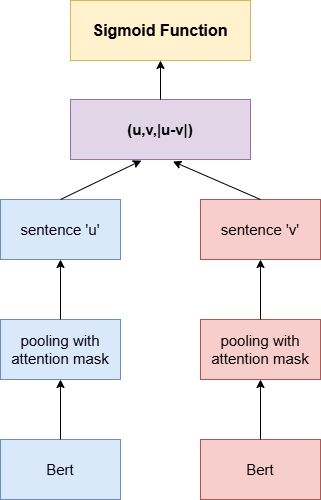
\includegraphics[width=0.6\linewidth]{Figures/SBERT_PD.png}
    \caption{SBERT Implementation Architecture for Paraphrase Detection. Referenced from \textit{Sentence-BERT: Sentence Embeddings using Siamese BERT-Networks} by Reimers and Gurevych~\cite{reimers2019sentence}}
    \label{fig:sbert_pd_architecture}
\end{figure}

\subsection{Semantic Textual Similarity (Regression Task)}

\textbf{Objective:} Estimate a continuous similarity score (0 to 5) that reflects how semantically close two sentences are.

\textbf{Embedding Interaction:} Sentence embeddings $u$ and $v$ are obtained using MEAN pooling and attention masking, as in the classification task.

\textbf{Similarity Computation:} Cosine similarity is computed between the two vectors:
\[
\text{sim}(u, v) = \frac{u^\top v}{\|u\| \cdot \|v\|}
\]
To match the STSb dataset scale (0 to 5), we use:
\[
\text{similarity} = \text{sim}(u, v) \times 2.5 + 2.5
\]

\textbf{Loss Function:} Mean Squared Error (MSE) loss is employed during training for this task:
\[
\mathcal{L}_{\text{regression}} = \frac{1}{N} \sum_{i=1}^{N} (s_i - \hat{s}_i)^2
\]
Where $s_i$ is the ground truth similarity score and $\hat{s}_i$ is the predicted similarity.

\textbf{Evaluation Metric - Pearson Correlation:}
Pearson Correlation measures the linear alignment between predicted and ground truth scores. Formula is
\[
r = \frac{\sum (x_i - \bar{x})(y_i - \bar{y})}{\sqrt{\sum (x_i - \bar{x})^2} \cdot \sqrt{\sum (y_i - \bar{y})^2}}
\]
where \( x_i \) denotes the predicted score, \( \bar{x} \) is the mean of the predicted scores, \( y_i \) is the ground truth score, \( \bar{y} \) is the mean of the ground truth scores, and \( r \) is the Pearson correlation coefficient.

Unlike MSE, Pearson correlation evaluates how well the model preserves the ranking of similarity across examples — which is the actual goal in STS.

\begin{figure}[H]
    \centering
    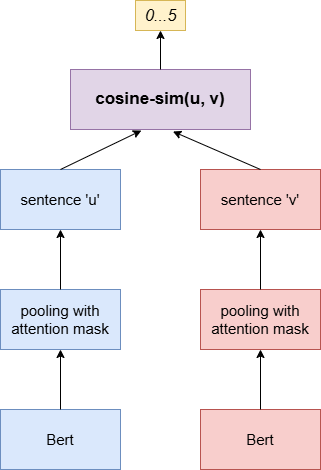
\includegraphics[height=10cm]{Figures/SBERT_STS.png}
    \caption{SBERT Implementation Architecture for Semantic Textual Similarity. Referenced from \textit{Sentence-BERT: Sentence Embeddings using Siamese BERT-Networks} by Reimers and Gurevych~\cite{reimers2019sentence}}
    \label{fig:sbert_sts_architecture}
\end{figure}

\subsection{Training Details}
The paraphrase detection model is trained using the QQP dataset with sigmoid activation and Binary Cross Entropy loss. The STS model is trained using the STSb dataset with cosine similarity and MSE loss. Dropout regularization is applied after pooling to prevent overfitting. Attention masking is consistently used to exclude padding tokens during pooling. Fine-tuning parameters such as learning rate and batch size are selected empirically to optimize performance.  

\chapter{Experimentation (Rooshan Khan)}
\label{Chapter4}
\lhead{Chapter 4. \emph{Experimentation}} % Write in your own chapter title to set the page header

\section{Phase 1}
Phase 1 of our project focused on fine-tuning BERT for the sentiment analysis task using the SST-5 and CFIMDB datasets. This phase aimed to understand the process of fine-tuning for a single task. We experimented with two fine-tuning strategies: (i) fine-tuning only the last linear layer, and (ii) fine-tuning the entire model. The development accuracies for both datasets under each strategy are presented in Table~\ref{tab:phase1_results}.
\begin{table}[H]
\centering
\caption{Quantitative Result of Phase 1. Accuracy comparison of BERT on SST and CFIMDB.}
\label{tab:phase1_results}
\begin{tabular}{l|cc|cc}
\toprule
 & \multicolumn{4}{c}{\textbf{Dev Accuracies}} \\
\midrule
 & \multicolumn{2}{c|}{\textbf{Ours}} & \multicolumn{2}{c}{\textbf{Reference}} \\
 & \textbf{SST} & \textbf{CFIMDB} & \textbf{SST} & \textbf{CFIMDB} \\
\midrule
last linear layer finetuning & 0.409 & 0.788 & 0.390 & 0.780 \\
full model finetuning        & 0.524 & 0.967 & 0.515 & 0.966 \\
\bottomrule
\end{tabular}
\end{table}

\section{Phase 2}
Imagine that we need separate models for different tasks. The biggest issue in this case is memory consumption. Storing 110 million parameters for each model becomes highly inefficient—n tasks would require n separate models, resulting in a total of 110n million parameters.

Why not use the same BERT model for all tasks? The question is: how? One approach is to share the 12 BERT layers across all tasks while using separate task-specific heads. This idea is illustrated in Figure~\ref{fig:Proposed Model}.
\begin{figure}[H]
    \centering
    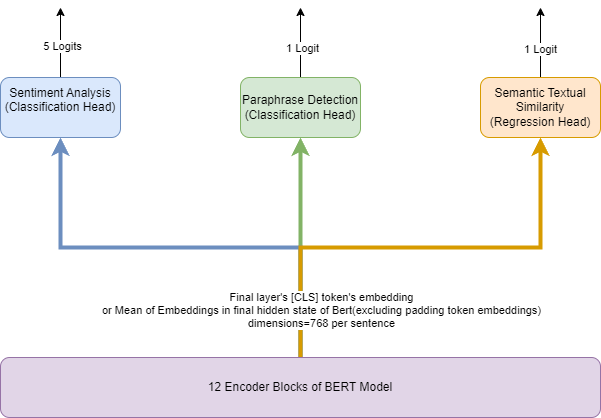
\includegraphics[width=0.8\linewidth]{Figures/Proposed_Model.png}
    \caption{Proposed Model}
    \label{fig:Proposed Model}
\end{figure}

We used Colab's L4 GPU for training and evaluating our models. Initially, we adopted a \texttt{batch\_size=32}, which worked well for baseline training. However, the introduction of SMART regularization significantly increased memory usage, leading to CUDA out-of-memory (OOM) errors.

For the Sentiment Analysis task, we were able to apply SMART successfully with \texttt{batch\_size=32} without encountering memory issues. However, for the Semantic Textual Similarity (STS) task, training with SMART triggered CUDA OOM errors, prompting us to lower the batch size to \texttt{16}.

Later, during training for the Paraphrase Detection task, we found that even \texttt{batch\_size=16} caused CUDA OOM errors. As a result, we further reduced the batch size to \texttt{8} for this task to ensure successful training.

The Architecture that we will be using throughout our experimentation is given in Figure~\ref{fig:Final_Model_Architecture}

\begin{figure}[H]
    \centering
    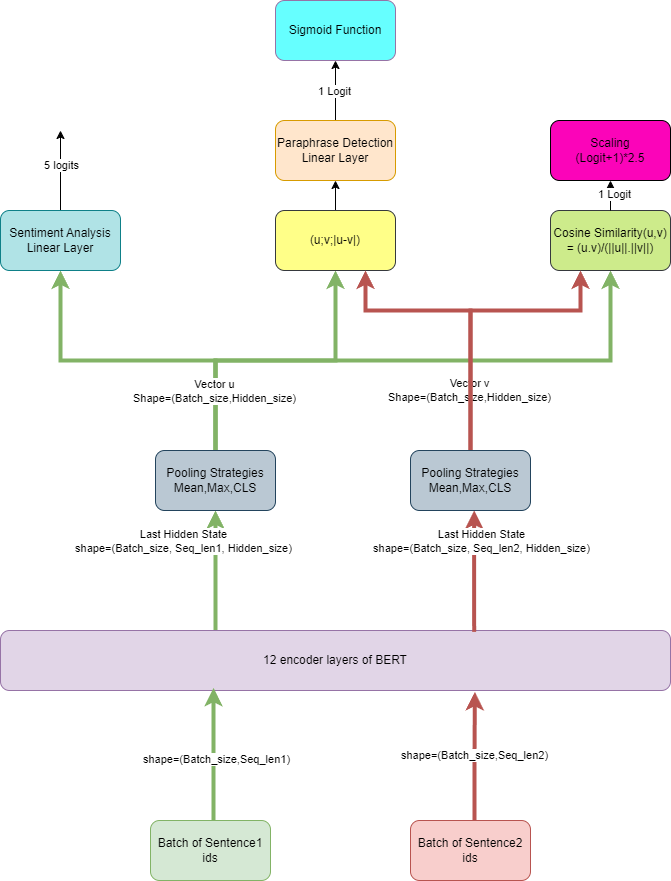
\includegraphics[width=0.8\linewidth]{Figures/Final Model Architecture.png}
    \caption{Final Model Architecture}
    \label{fig:Final_Model_Architecture}
\end{figure}


\subsection{Individually fine-tuned BERT models}
\label{subsec:Individually fine-tuned BERT models}
We first trained and tested our models on individual tasks. The best accuracy on the SST dataset was achieved using the mean of all vectors from the last hidden state corresponding to the input words (excluding padding tokens). We employed the SMART algorithm for training. The highest accuracy obtained was \textbf{0.533} at \textbf{epoch 7}. We set the hyperparameters as follows: \(\lambda_s = 10\) and \(\mu = 1\). A dropout rate of 0.3 was used during training. Look at Figure~\ref{fig:sst_accuracy}.
\begin{figure}[H]
    \centering
    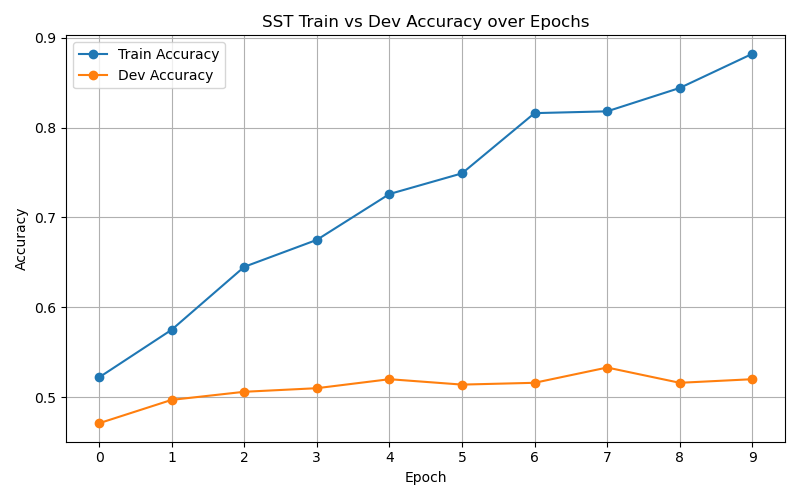
\includegraphics[width=0.8\linewidth]{Figures/sst_accuracy_plot.png}
    \caption{SST train vs dev accuracy over 10 epochs}
    \label{fig:sst_accuracy}
\end{figure}

When we trained our model on the Semantic Textual Similarity (STS) task alone, we achieved a best Pearson correlation of 0.821 on the development set. We achieved Pearson correlation on the first epoch. We used SBERT architecture with mean pooling for regression tasks that finds cosine similarity between sentences. We shifted and scaled this cosine similarity to be in the range from 0 to 5 instead of -1 to 1. We also used the SMART algorithm during training. We used $\lambda_s=5$ and $\mu=1$. A dropout rate of 0.3 was used during training. As shown in Figure~\ref{fig:sts_corr}, the dev STS correlation starts to drop after epoch 0, indicating potential overfitting.

\begin{figure}[H]
    \centering
    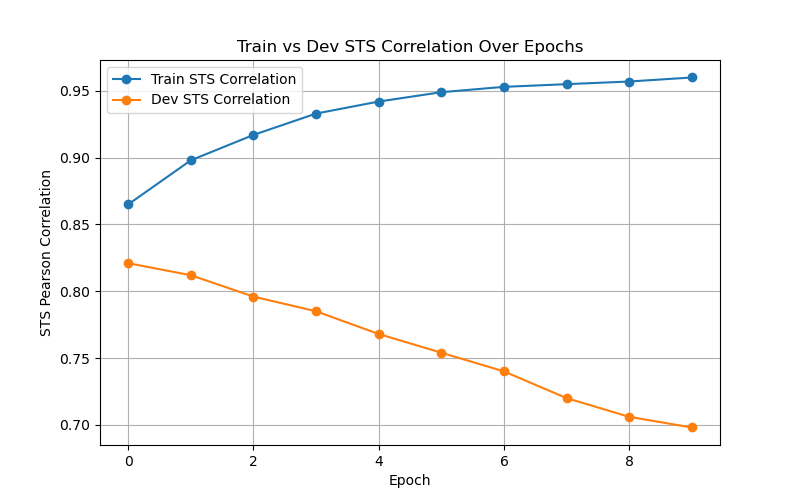
\includegraphics[width=0.8\linewidth]{Figures/sts_corr_plot.png}
    \caption{STS train vs dev correlation over 10 epochs}
    \label{fig:sts_corr}
\end{figure}

For the Paraphrase Detection task, our model achieved a maximum accuracy of 0.875 with hyperparameters set to $\lambda_s = 5$ and $\mu = 1$. Due to computational constraints, we trained the model for only one epoch. Specifically, incorporating SMART significantly increased training time to approximately 5 hours per epoch, which was not feasible given our limited compute resources. A dropout rate of 0.1 was used during training. Batch size was set to 8 to avoid CUDA out-of-memory error.  We used SBERT architecture with mean pooling for this classification task.

The results for separate models trained individually for each task are summarized in Table~\ref{tab:smart_per_task}.

\begin{table}[H]
    \centering
    \begin{tabular}{|l|l|c|}
    \hline
    \textbf{Task} & \textbf{Metric} & \textbf{Value} \\ 
    \hline
    Sentiment Classification (SST-5) & Accuracy & 0.533 \\ 
    \hline
    Paraphrase Detection (QQP) & Accuracy & 0.875 \\ 
    \hline
    Semantic Textual Similarity (STS-B) & Pearson Correlation & 0.821 \\ 
    \hline
    \end{tabular}
    \caption{Best performance of separate models fine-tuned individually for each task}
    \label{tab:smart_per_task}
\end{table}


% \begin{table}[h]
%     \centering
%     \caption{Performance with SMART Fine-Tuning Applied Independently per Task}
%     \label{tab:smart_per_task}
%     \begin{tabular}{|l|c|}
%     \hline
%     \textbf{Task} & \textbf{Best Metric Value} \\
%     \hline
%     Sentiment Classification (SST-5) Accuracy & 0.533 \\
%     Paraphrase Detection (QQP) Accuracy & 0.875 \\
%     Semantic Textual Similarity (STS-B) Pearson Correlation & 0.821 \\
%     \hline
%     \end{tabular}
% \end{table}

\subsection{Accuracies and Pearson Correlation for Fine-Tuning the same model on Multiple Tasks}
\subsubsection{Sequential Fine-Tuning: SBERT Only}

We trained the model for \textbf{3} epochs on the Paraphrase Detection task, \textbf{10} epochs on the Semantic Textual Similarity (STS) task, and \textbf{10} epochs on the Sentiment Analysis task.

\begin{table}[H]
    \centering
    \begin{tabular}{|l|l|c|}
    \hline
    \textbf{Task} & \textbf{Metric} & \textbf{Value} \\ \hline
    Paraphrase Detection & Accuracy & 0.6285 \\ \hline
    Semantic Textual Similarity (STS) & Pearson Correlation & 0.5444 \\ \hline
    Sentiment Analysis (SST) & Accuracy & 0.1698 \\ \hline
    \end{tabular}
    \caption{Development set performance before fine-tuning}
    \label{tab:pre_finetuning_metrics}
\end{table}

After training for 3 epochs on the QQP dataset, the best Paraphrase Detection accuracy achieved was \textbf{0.7441}. See Figure~\ref{fig:paraphrase_acc_plot} for the training and development curves.

\begin{figure}[H]
    \centering
    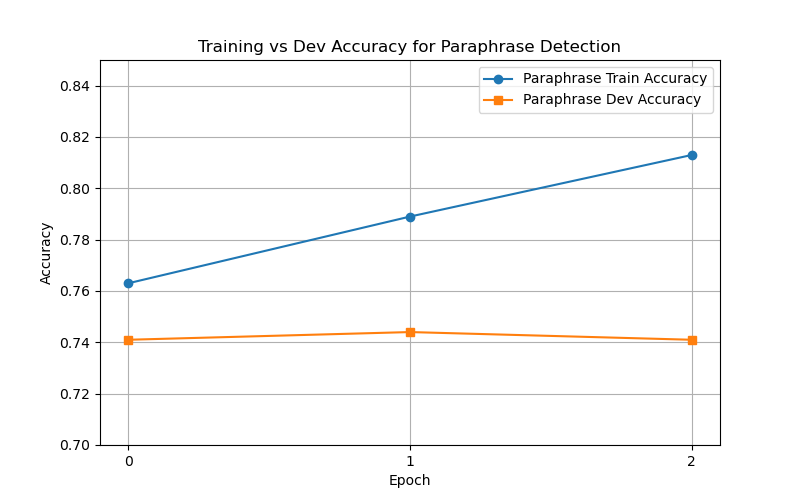
\includegraphics[width=0.8\textwidth]{Figures/Paraphrase_plot_3epochs_SBERT_Only.png}
    \caption{Train vs Dev Accuracy for Paraphrase Detection using SBERT Only (3 epochs)}
    \label{fig:paraphrase_acc_plot}
\end{figure}

\begin{table}[H]
    \centering
    \begin{tabular}{|l|l|c|}
    \hline
    \textbf{Task} & \textbf{Metric} & \textbf{Value} \\ \hline
    Paraphrase Detection & Accuracy & 0.7441 \\ \hline
    Semantic Textual Similarity (STS) & Pearson Correlation & 0.7127 \\ \hline
    Sentiment Analysis (SST) & Accuracy & 0.1735 \\ \hline
    \end{tabular}
    \caption{Development set performance after fine-tuning on Paraphrase Detection for 3 epochs}
    \label{tab:post_finetuning_paraphrase_metrics}
\end{table}

Subsequently, we fine-tuned the best-performing model for \textbf{10} epochs on the STS task.

\begin{figure}[H]
    \centering
    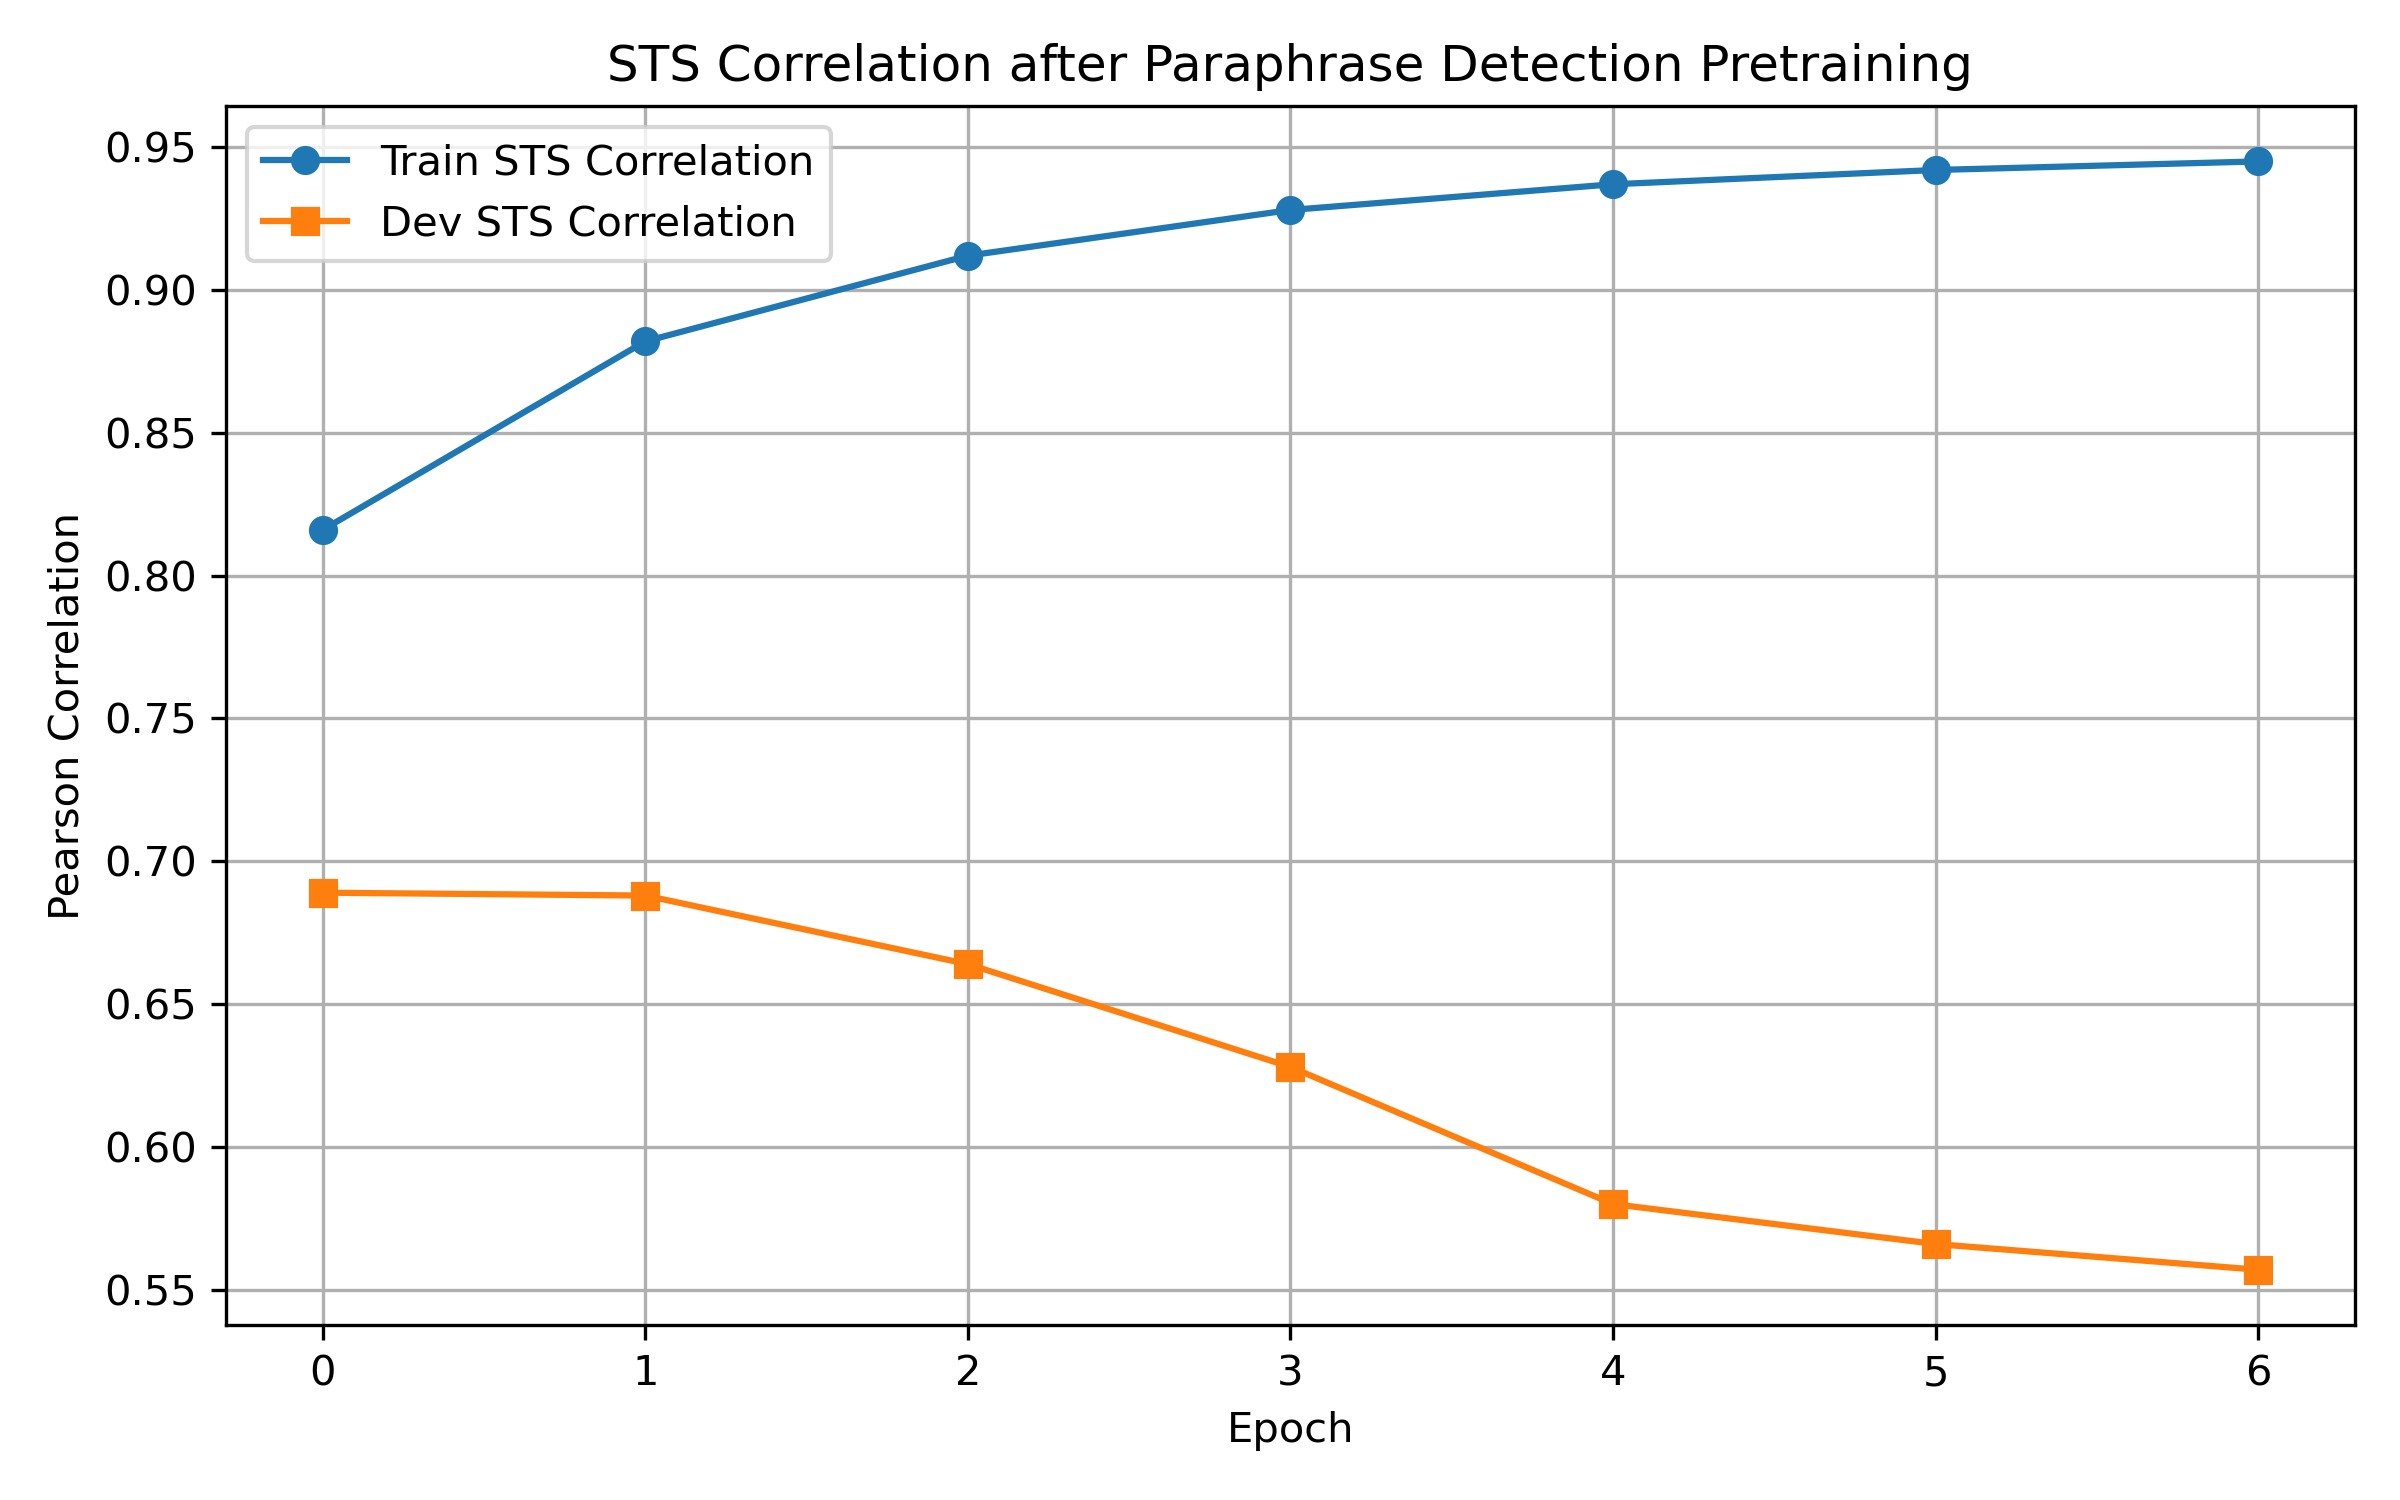
\includegraphics[width=0.6\textwidth]{Figures/STS_plot_10epochs_SBERT_Only.png}
    \caption{Train vs Dev Correlation for Semantic Textual Similarity using SBERT Only (10 epochs)}
    \label{fig:sts_corr_plot}
\end{figure}

\begin{table}[H]
    \centering
    \begin{tabular}{|l|l|c|}
    \hline
    \textbf{Task} & \textbf{Metric} & \textbf{Value} \\ \hline
    Paraphrase Detection & Accuracy & 0.8353 \\ \hline
    Semantic Textual Similarity (STS) & Pearson Correlation & 0.6890 \\ \hline
    Sentiment Analysis (SST) & Accuracy & 0.1835 \\ \hline
    \end{tabular}
    \caption{Development set performance after fine-tuning on the STS task}
    \label{tab:post_finetuning_sts_metrics}
\end{table}

Finally, we fine-tuned the best-performing model for \textbf{10} epochs on the Sentiment Analysis task.

\begin{figure}[H]
    \centering
    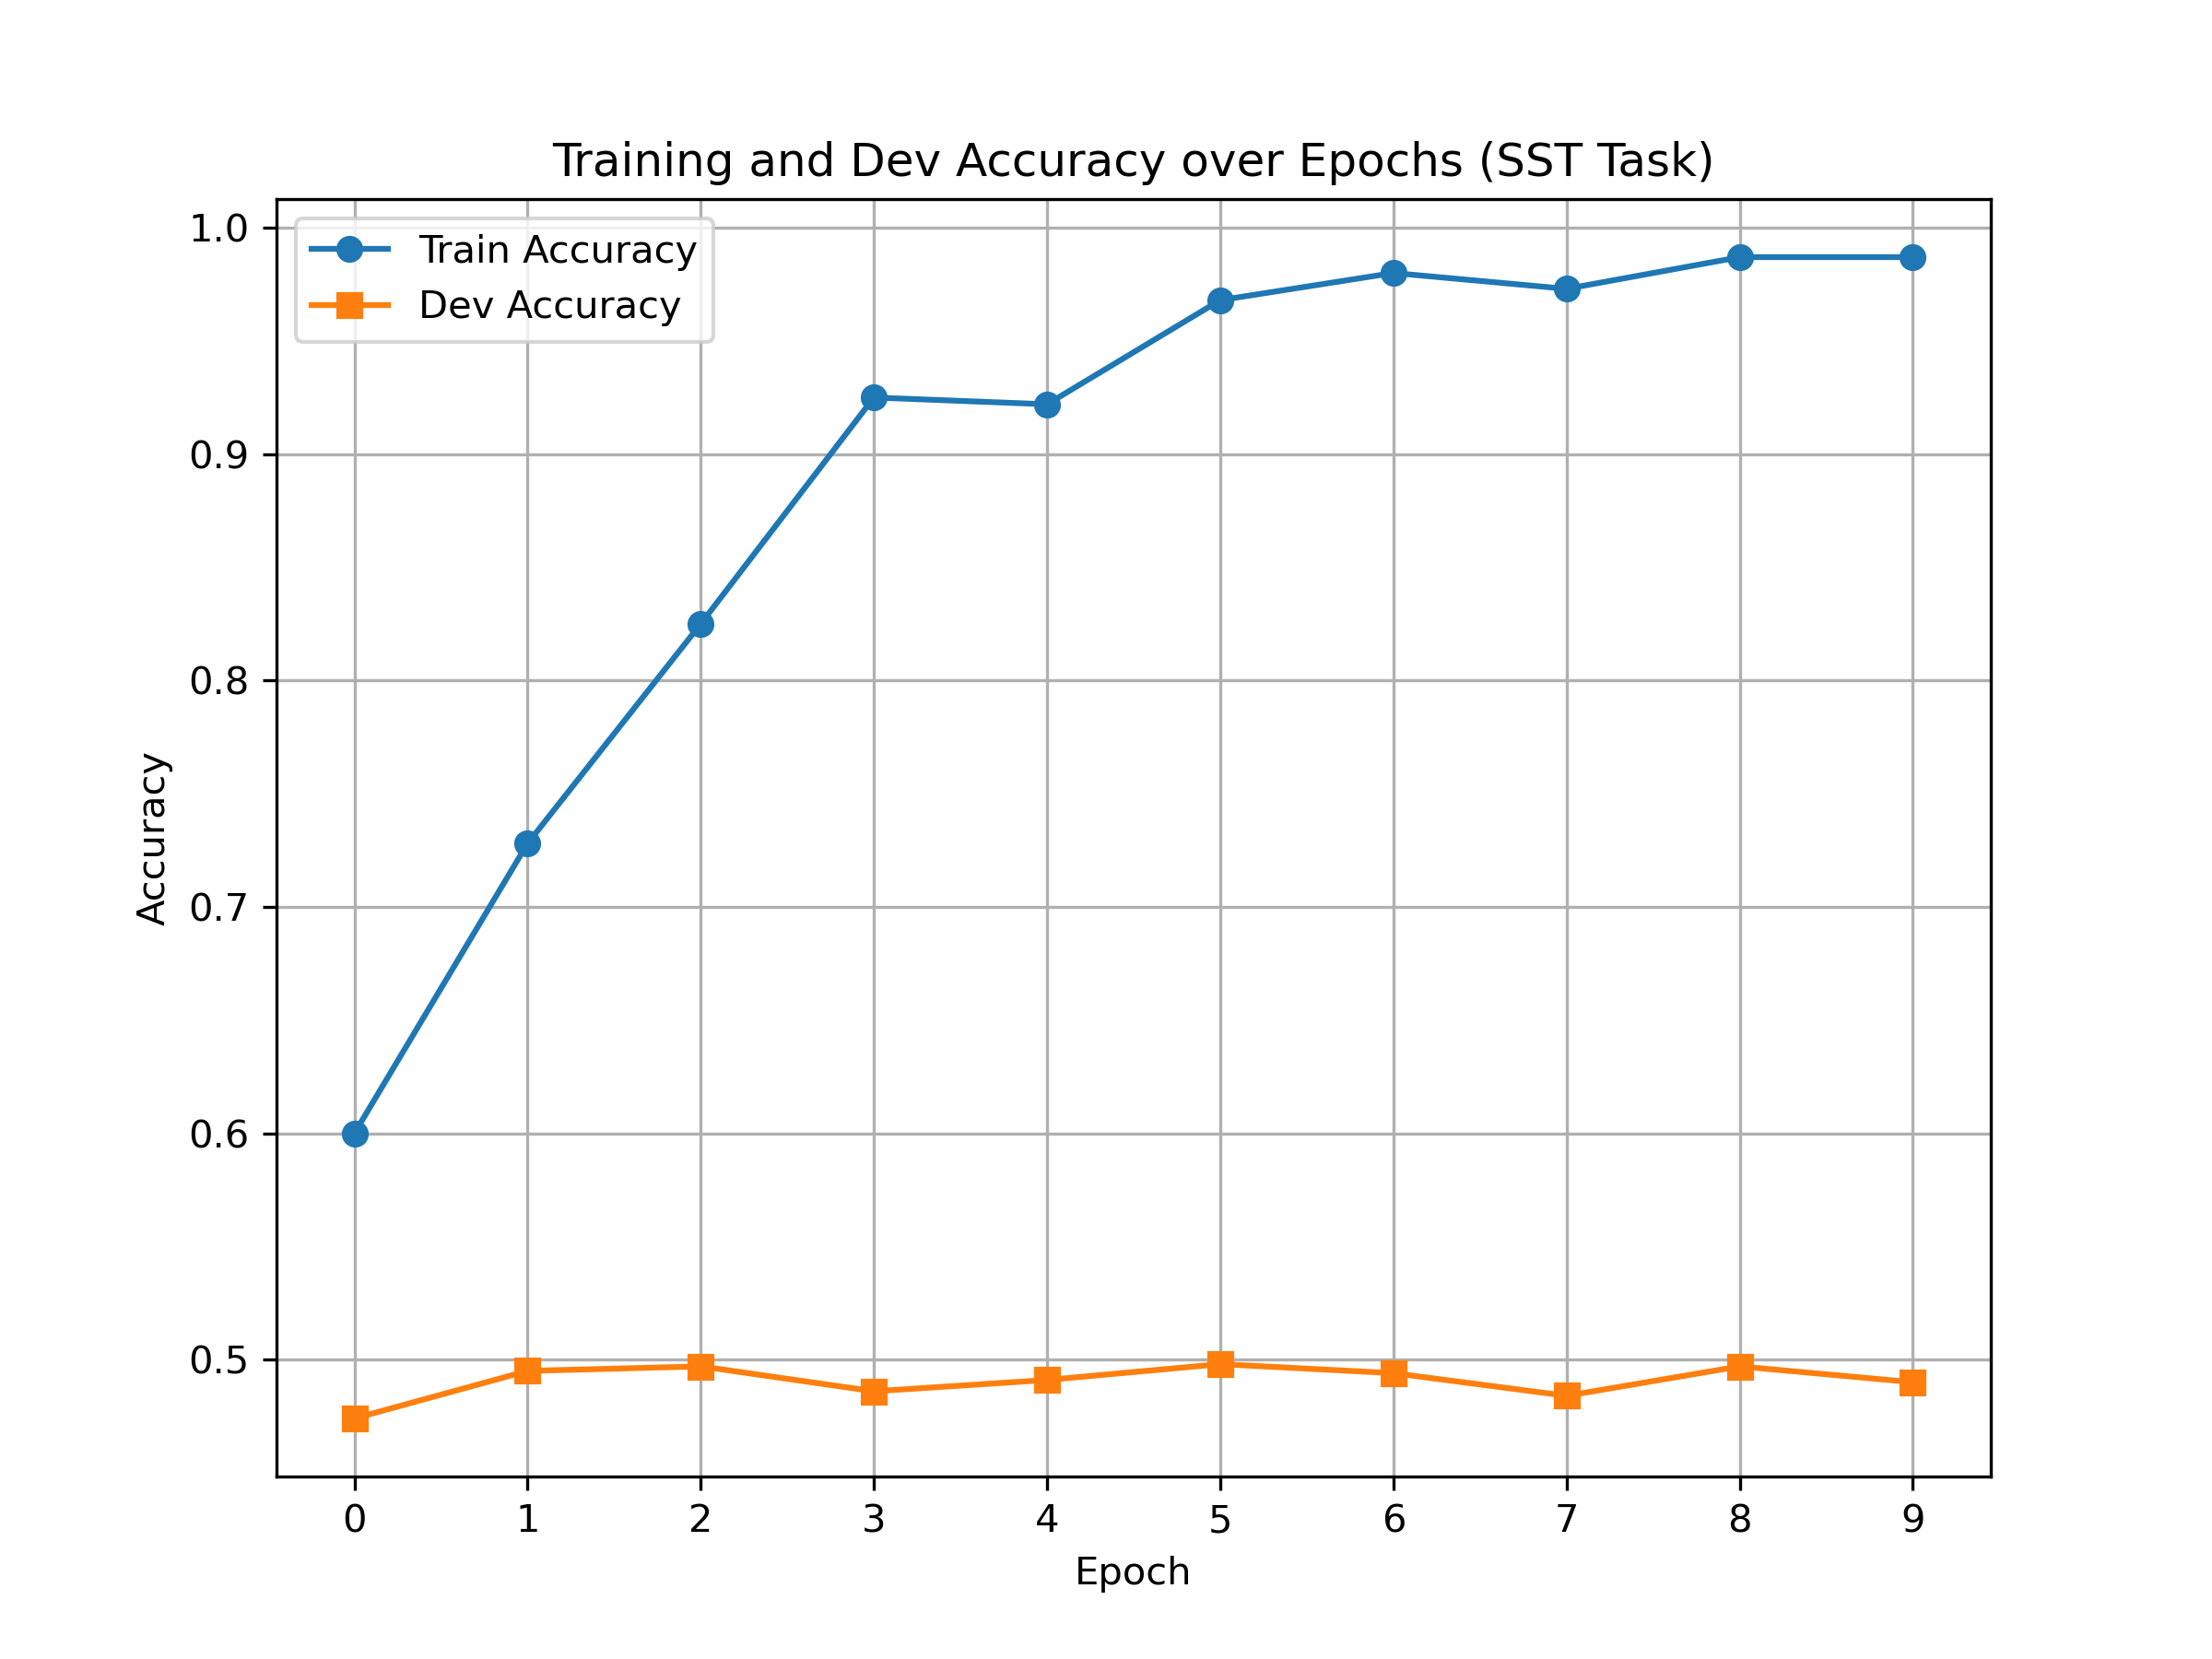
\includegraphics[width=0.7\textwidth]{Figures/SST_plot_10epochs_SBERT_Only.png}
    \caption{Train vs Dev Accuracy for Sentiment Analysis using SBERT Only (10 epochs)}
    \label{fig:sst_acc_plot}
\end{figure}

\begin{table}[H]
    \centering
    \begin{tabular}{|l|l|c|}
    \hline
    \textbf{Task} & \textbf{Metric} & \textbf{Value} \\ \hline
    Paraphrase Detection & Accuracy & 0.7940 \\ \hline
    Semantic Textual Similarity (STS) & Pearson Correlation & 0.6220 \\ \hline
    Sentiment Analysis (SST) & Accuracy & 0.4980 \\ \hline
    \end{tabular}
    \caption{Development set performance after fine-tuning for 10 epochs on SST}
    \label{tab:post_finetuning_metrics}
\end{table}

\begin{itemize}
    \item \textbf{Observations:}
    We observed that training on each task could negatively impact the performance on dissimilar tasks. For example, training on the SST task hurt the model's performance on the STS task. In contrast, training on a particular task improved performance on related tasks. For instance, fine-tuning the model for paraphrase detection improved the correlation score on the STS task, while training on the STS task enhanced the accuracy on the paraphrase detection task.
\end{itemize}

\subsubsection{Sequential Fine-Tuning: SBERT+SMART}
For this training paradigm, we were constrained to use a batch size of 8 due to CUDA out-of-memory errors for higher batch sizes. The SMART regularization technique significantly slowed down training. Specifically, the paraphrase detection task failed for batch sizes above 8. Hence, we decided to use a uniform batch size of 8 across all tasks.

Fine-tuning for paraphrase detection (QQP) took approximately 5 hours per epoch. Due to limited computational resources, we fine-tuned for only one epoch. The development accuracy obtained after this epoch was 0.807. The resulting metrics for all three tasks are summarized in Table~\ref{tab:post_finetuning_metrics_SS}.

\begin{table}[H]
    \centering
    \begin{tabular}{|l|l|c|}
    \hline
    \textbf{Task} & \textbf{Metric} & \textbf{Value} \\ \hline
    Paraphrase Detection & Accuracy & 0.8067 \\ \hline
    Semantic Textual Similarity (STS) & Pearson Correlation & 0.7567 \\ \hline
    Sentiment Analysis (SST) & Accuracy & 0.2089 \\ \hline
    \end{tabular}
    \caption{Development set performance after fine-tuning on Paraphrase Detection for 1 epoch}
    \label{tab:post_finetuning_metrics_SS}
\end{table}

Subsequently, we fine-tuned the model on the STS dataset for 10 epochs. Interestingly, we observed that the highest Pearson correlation was achieved in the first epoch, followed by a consistent decline. This trend is shown in Figure~\ref{fig:SS_sts_corr}.

\begin{figure}[H]
    \centering
    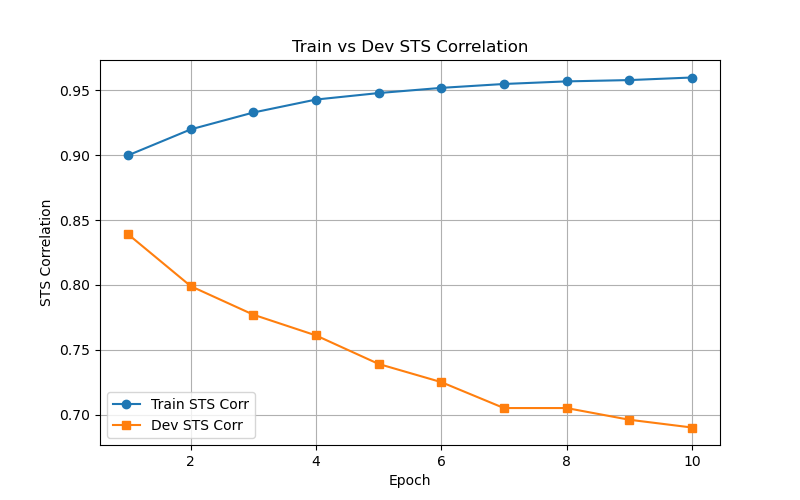
\includegraphics[width=0.7\textwidth]{Figures/SS_sts_corr.png}
    \caption{Train vs Dev Pearson Correlation for STS using SMART SBERT (10 epochs)}
    \label{fig:SS_sts_corr}
\end{figure}

The post-training metrics for all tasks are listed below.

\begin{table}[H]
    \centering
    \begin{tabular}{|l|l|c|}
    \hline
    \textbf{Task} & \textbf{Metric} & \textbf{Value} \\ \hline
    Paraphrase Detection & Accuracy & 0.8045 \\ \hline
    Semantic Textual Similarity (STS) & Pearson Correlation & 0.8394 \\ \hline
    Sentiment Analysis (SST) & Accuracy & 0.2044 \\ \hline
    \end{tabular}
    \caption{Development set performance after fine-tuning for 10 epochs on STS}
    \label{tab:post_finetuning_metrics_SS2}
\end{table}

Finally, we fine-tuned the best model from the STS stage on the SST dataset for 10 epochs. The train vs. dev accuracy trends are illustrated in Figure~\ref{fig:SS_sst_acc}.

\begin{figure}[H]
    \centering
    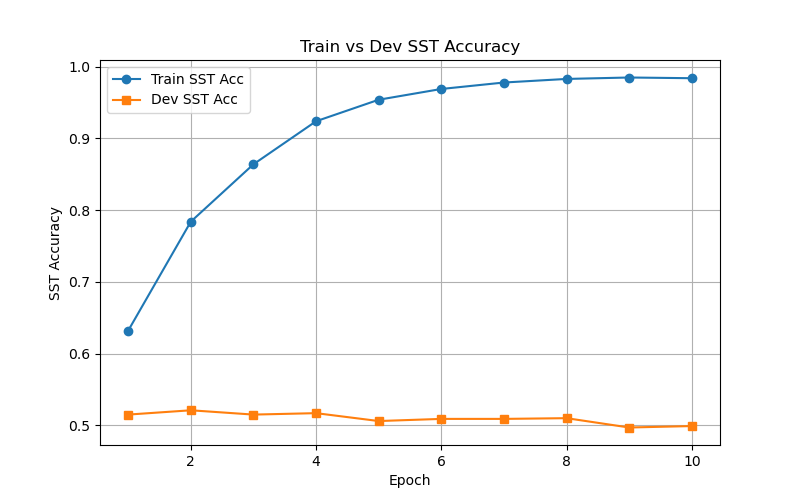
\includegraphics[width=0.7\textwidth]{Figures/SS_sst_acc.png}
    \caption{Train vs Dev Accuracy for SST using SMART SBERT (10 epochs)}
    \label{fig:SS_sst_acc}
\end{figure}

The resulting performance metrics are reported in Table~\ref{tab:post_finetuning_metrics_SS3}.

\begin{table}[H]
    \centering
    \begin{tabular}{|l|l|c|}
    \hline
    \textbf{Task} & \textbf{Metric} & \textbf{Value} \\ \hline
    Paraphrase Detection & Accuracy & 0.7350 \\ \hline
    Semantic Textual Similarity (STS) & Pearson Correlation & 0.7880 \\ \hline
    Sentiment Analysis (SST) & Accuracy & 0.5210 \\ \hline
    \end{tabular}
    \caption{Development set performance after fine-tuning for 10 epochs on SST}
    \label{tab:post_finetuning_metrics_SS3}
\end{table}
We changed the dropout to 0.1 and found that after training for 1 epoch on the paraphrase detection task, the accuracy reached 0.8749. However, when we trained this model on the STS task, the accuracy for STS rose to 0.8580, but the paraphrase detection accuracy dropped to 0.7523. This was due to catastrophic forgetting. Therefore, we decided to train the model as follows:

\begin{enumerate}
    \item Train the model for one epoch on the paraphrase task using the complete dataset.
    \item Train the model for one epoch on the STS dataset (full dataset).
    \item Train the model for one epoch on the SST dataset (full dataset).
    \item Train the model on the paraphrase task using only 3\% of the dataset.
\end{enumerate}

We repeat steps 2 to 4 ten times and save the best model. Overall performance is calculated after training on each task using the following formula:
\[
\text{Overall performance} = \frac{\left( \frac{\text{dev\_sts\_corr} + 1}{2} + \text{sst\_dev\_acc} + \text{paraphrase\_dev\_acc} \right)}{3}
\]

This updated training procedure can be seen in Figure~\ref{fig:Training_Procedure}.

\begin{figure}[H]
    \centering
    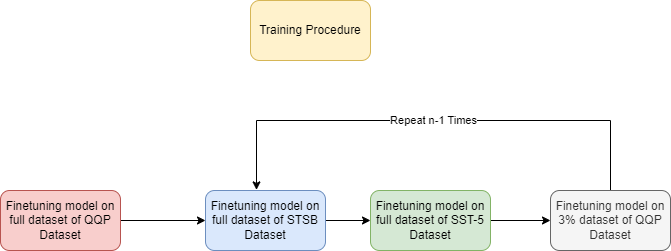
\includegraphics[width=0.7\textwidth]{Figures/Training_Procedure.png}
    \caption{Updated Training Procedure}
    \label{fig:Training_Procedure}
\end{figure}


The optimal model is the one with the highest overall performance across all tasks.

The following table shows the metrics for our best model so far:

\begin{table}[H]
    \centering
    \begin{tabular}{|l|l|c|}
    \hline
    \textbf{Task} & \textbf{Metric} & \textbf{Score} \\
    \hline
    Sentiment Classification & Accuracy & 0.537 \\
    & F1 Score & 0.528 \\
    \hline
    Paraphrase Detection & Accuracy & 0.864 \\
    & F1 Score & 0.864 \\
    \hline
    Semantic Textual Similarity & Pearson Correlation & 0.819 \\
    \hline
    \end{tabular}
    \caption{Evaluation metrics for each task (SMART+SBERT)}
\end{table}
    
Since we changed the training procedure and dropout (from 0.3 to 0.1), it seems logical to retrain the \texttt{SBERT\_Only} model using the new procedure and dropout for a fair comparison.\\
We obtain the following results:

\begin{table}[H]
    \centering
    \begin{tabular}{|l|l|c|}
    \hline
    \textbf{Task} & \textbf{Metric} & \textbf{Score} \\
    \hline
    Sentiment Classification & Accuracy & 0.501 \\
    & F1 Score & 0.495 \\
    \hline
    Paraphrase Detection & Accuracy & 0.854 \\
    & F1 Score & 0.856 \\
    \hline
    Semantic Textual Similarity & Pearson Correlation & 0.680 \\
    \hline
    \end{tabular}
    \caption{Evaluation metrics for each task (SBERT Only)}
\end{table}

\subsubsection{Sequentual Fine-Tuning: SBERT+SimCSE+SMART}
Before applying the training procedure shown in Figure~\ref{fig:Training_Procedure}, we performed contrastive loss minimization (Supervised SimCSE Loss) on the SNLI dataset for 3 epochs, as recommended in \textit{SimCSE: Simple Contrastive Learning of Sentence Embeddings} by Gao et al.~\cite{gao2021simcse}. The best model was selected based on the highest Pearson correlation on the STS-B task. Sentence embeddings were computed as the mean of the token embeddings from the last layer of BERT.
We obtain the following results after this step:
\begin{table}[H]
\centering
\begin{tabular}{|l|l|c|}
\hline
\textbf{Task} & \textbf{Metric} & \textbf{Score} \\
\hline
Sentiment Classification & Accuracy & 0.221 \\
& F1 Score & 0.174 \\
\hline
Paraphrase Detection & Accuracy & 0.626 \\
& F1 Score & 0.503 \\
\hline
Semantic Textual Similarity & Pearson Correlation & 0.812 \\
\hline
\end{tabular}
\caption{Evaluation metrics for each task}
\end{table}

Then after this we begin the training procedure of Figure~\ref{fig:Training_Procedure}. When we train the model for 1 complete QQP datset we get an accuracy of 0.876. However, with the later training we could reach a maximum performance of 0.764. This is lower than what we got for SMART SBERT (Our best model so far).
The results are shown in the table below.

\begin{table}[H]
\centering
\begin{tabular}{|l|l|c|}
\hline
\textbf{Task} & \textbf{Metric} & \textbf{Score} \\
\hline
Sentiment Classification & Accuracy & 0.507 \\
& F1 Score & 0.494 \\
\hline
Paraphrase Detection & Accuracy & 0.864 \\
& F1 Score & 0.863 \\
\hline
Semantic Textual Similarity & Pearson Correlation & 0.843 \\
\hline
\multicolumn{2}{|l|}{\textbf{Overall Performance}} & 0.764 \\
\hline
\end{tabular}
\caption{Evaluation metrics for each task}
\end{table}

\section{Analysis of the Results}
Our best-performing model achieved an overall score of 0.770\%. These results are in line with the top-performing individual models (developed by us) discussed in Section~\ref{subsec:Individually fine-tuned BERT models}. Additionally, our outcomes are competitive with state-of-the-art results reported for each task. The benchmark scores listed in Table~\ref{tab:bert-sota-clean} are sourced from \textit{Papers with Code}~\cite{paperswithcode}.

\begin{table}[H]
\centering
\begin{tabular}{|l|l|c|}
\hline
\textbf{Task} & \textbf{Metric} & \textbf{Score} \\
\hline
Sentiment Classification & Accuracy & 0.532 \\
\hline
Paraphrase Detection & Accuracy & 0.910 \\
\hline
Semantic Textual Similarity & Pearson Correlation & 0.8479 \\
\hline
\multicolumn{2}{|l|}{\textbf{Overall Performance}} & 0.7887 \\
\hline
\end{tabular}
\caption{State-of-the-art BERT-base results for each task}
\label{tab:bert-sota-clean}
\end{table}

We have two strong models: SMART SBERT (SS) and SMART SBERT with SimCSE (SSS). Both SS and SSS perform approximately equally well on the paraphrase detection task. However, SS performs better on the SST-5 task, while SSS performs better on the STS-B task. The superior performance of SSS on STS-B is understandable, as the supervised SimCSE loss is specifically optimized to enhance performance on semantic textual similarity tasks such as STS-B. Depending on the task priority, either of the two models can be selected.

\chapter{Possible Improvements (Areesha Noor)}
\label{Chapter6}
\lhead{Chapter 6. \emph{Possible Improvements}}

% The Quora Question Pairs (QQP) dataset is imbalanced, with approximately 63\% of the examples labeled as non-duplicates and 37\% as duplicates in both the training and validation splits. Despite this imbalance, we used accuracy as the primary evaluation metric and based all model selection and checkpointing decisions on it. 

% To better account for class imbalance, we also computed the F$_1$ score, which combines precision and recall to provide a more balanced view of binary classification performance. However, we did not use it for selecting the best model.

% The definitions are as follows:
% \begin{align}
% \text{Precision} &= \frac{\text{TP}}{\text{TP} + \text{FP}}, \\
% \text{Recall}    &= \frac{\text{TP}}{\text{TP} + \text{FN}}, \\
% F_1              &= 2 \times \frac{\text{Precision} \times \text{Recall}}{\text{Precision} + \text{Recall}},
% \end{align}
% where TP, FP, and FN represent the number of true positives, false positives, and false negatives, respectively.

% \section{Class Imbalance in SST-5}
% Similar to the Quora Question Pairs dataset, the SST-5 dataset is also imbalanced, where the class distribution changes significantly across five sentiment categories. In the training split dataset, the most frequent classes are \textit{Positive} and \textit{Negative}, making 27.4\% and 26\% of the total dataset respectively. Whereas, \textit{Very Positive} and \textit{Very Negative} classes contain only 15.1\% and 12.8\% of the total data.

% \section{Need for Weighted F1 Score}
% Given the imbalanced class distribution, using accuracy as a metric may not provide an accurate assessment of the model's performance as it could heavily rely on majority classes. Therefore, similar to the Quora Question Pairs dataset, we use the sample-weighted F1 score for SST-5 to better evaluate performance across all classes. This metric combines two important competing metrics:

% \begin{align*}
% \text{Precision} &= \frac{TP}{TP + FP} \\
% \text{Recall} &= \frac{TP}{TP + FN}
% \end{align*}

% where:
% \begin{itemize}
%     \item $TP$ is the number of true positives
%     \item $FP$ is the number of false positives
%     \item $FN$ is the number of false negatives
% \end{itemize}

% \section{Calculating Weighted F1 Score}
% The sample-weighted F1 score helps by weighing each class's F1 score based on its true instances. The calculation involves two steps:

% \subsection{Class-wise F1 Scores}
% First, we compute F1 scores for each class individually:
% \[
% F1_i = 2 \times \frac{\text{Precision}_i \times \text{Recall}_i}{\text{Precision}_i + \text{Recall}_i}
% \]

% \subsection{Weighted Average}
% Then, we calculate the weighted average across all classes:
% \[
% \text{Weighted F1 Score} = \sum_{i=1}^{N} w_i \times F1_i
% \]
% where $w_i = \frac{\text{Number of samples in class } i}{\text{Total number of samples}}$.

% \section{Python Implementation}
% In our implementation, we modified the evaluation function by changing:
% \begin{verbatim}
% f1_score(y_true, y_pred, average='macro')
% \end{verbatim}
% to:
% \begin{verbatim}
% f1_score(y_true, y_pred, average='weighted')
% \end{verbatim}

% This change makes the function:
% \begin{itemize}
%     \item Compute class-wise F1 scores
%     \item Weight them by their class support (number of true instances)
%     \item Provide more realistic performance metrics for imbalanced datasets
% \end{itemize}

% The weighted F1 score proves particularly suitable for imbalanced datasets like SST-5 and Quora Question Pairs, as it provides more balanced evaluation performance by appropriately weighting each class's contribution.

The Quora Question Pairs (QQP) dataset used is imbalanced, containing approximately 63\% of the examples labeled as non-duplicates and 37\% as duplicates, in both training and validation splits. Despite this imbalance, we used \textbf{accuracy} as the primary evaluation metric and based our model selection on it. This is mainly to make a fair comparison among our models, as state-of-the-art results also use this metric.

To better account for class imbalance, the accuracy metric may not be a reliable metric as it provides an overall performance score. Instead, we can focus on computing the \textbf{sample-weighted F1 score}.

Similar to the Quora Question Pairs dataset, the SST-5 dataset is also imbalanced, where the class distribution changes significantly across five sentiment categories. In the training split dataset, the most frequent classes are \textit{Positive} and \textit{Negative}, making up 27.4\% and 26\% of the total dataset, respectively. Meanwhile, \textit{Very Positive} and \textit{Very Negative} classes contain only 15.1\% and 12.8\% of the total data, respectively.

Given the imbalanced class distribution for the above datasets, using the accuracy metric may not provide an accurate assessment of a model's performance, as it could heavily rely on majority classes. So, like the QQP dataset, here also, the \textbf{sample-weighted F1 score} could be used for the SST-5 dataset to better evaluate performance across all classes. It considers two competing metrics: precision and recall.

\begin{align*}
\text{Precision} &= \frac{TP}{TP + FP} \\
\text{Recall} &= \frac{TP}{TP + FN}
\end{align*}

\noindent where:
\begin{itemize}
    \item TP is the number of true positives
    \item FP is the number of false positives
    \item FN is the number of false negatives
\end{itemize}

Sample F1 score helps by weighing the F1 score for each class on the basis of its true instances. First, we compute class-wise F1 scores as:

\[
F1 = \frac{2 \times \text{Precision} \times \text{Recall}}{\text{Precision} + \text{Recall}}
\]

Then, we take the weighted average of F1 scores for all classes as:

\[
\text{Weighted F1 Score} = \sum_{i=1}^{N} w_i \times F1_i
\]

\noindent where:
\[
w_i = \frac{\text{Number of samples in class } i}{\text{Total number of samples}}
\]

Here, the sample-weighted F1 score provides a more balanced evaluation by equitably weighing each class and thus proves more suitable for imbalanced datasets like SST-5.

In our Python implementation, we modified one parameter in the evaluation function by changing:

\begin{verbatim}
f1_score(y_true, y_pred, average='macro')
\end{verbatim}

to

\begin{verbatim}
f1_score(y_true, y_pred, average='weighted')
\end{verbatim}

This computes class-wise F1 scores and then multiplies them by their weights (number of true instances). This approach helps in providing more realistic performance evaluation in the case of imbalanced datasets like SST-5 or Quora Question Pairs.

%\chapter{Possible Improvements (Areesha Noor)}
\label{Chapter6}
\lhead{Chapter 6. \emph{Possible Improvements}}

% The Quora Question Pairs (QQP) dataset is imbalanced, with approximately 63\% of the examples labeled as non-duplicates and 37\% as duplicates in both the training and validation splits. Despite this imbalance, we used accuracy as the primary evaluation metric and based all model selection and checkpointing decisions on it. 

% To better account for class imbalance, we also computed the F$_1$ score, which combines precision and recall to provide a more balanced view of binary classification performance. However, we did not use it for selecting the best model.

% The definitions are as follows:
% \begin{align}
% \text{Precision} &= \frac{\text{TP}}{\text{TP} + \text{FP}}, \\
% \text{Recall}    &= \frac{\text{TP}}{\text{TP} + \text{FN}}, \\
% F_1              &= 2 \times \frac{\text{Precision} \times \text{Recall}}{\text{Precision} + \text{Recall}},
% \end{align}
% where TP, FP, and FN represent the number of true positives, false positives, and false negatives, respectively.

% \section{Class Imbalance in SST-5}
% Similar to the Quora Question Pairs dataset, the SST-5 dataset is also imbalanced, where the class distribution changes significantly across five sentiment categories. In the training split dataset, the most frequent classes are \textit{Positive} and \textit{Negative}, making 27.4\% and 26\% of the total dataset respectively. Whereas, \textit{Very Positive} and \textit{Very Negative} classes contain only 15.1\% and 12.8\% of the total data.

% \section{Need for Weighted F1 Score}
% Given the imbalanced class distribution, using accuracy as a metric may not provide an accurate assessment of the model's performance as it could heavily rely on majority classes. Therefore, similar to the Quora Question Pairs dataset, we use the sample-weighted F1 score for SST-5 to better evaluate performance across all classes. This metric combines two important competing metrics:

% \begin{align*}
% \text{Precision} &= \frac{TP}{TP + FP} \\
% \text{Recall} &= \frac{TP}{TP + FN}
% \end{align*}

% where:
% \begin{itemize}
%     \item $TP$ is the number of true positives
%     \item $FP$ is the number of false positives
%     \item $FN$ is the number of false negatives
% \end{itemize}

% \section{Calculating Weighted F1 Score}
% The sample-weighted F1 score helps by weighing each class's F1 score based on its true instances. The calculation involves two steps:

% \subsection{Class-wise F1 Scores}
% First, we compute F1 scores for each class individually:
% \[
% F1_i = 2 \times \frac{\text{Precision}_i \times \text{Recall}_i}{\text{Precision}_i + \text{Recall}_i}
% \]

% \subsection{Weighted Average}
% Then, we calculate the weighted average across all classes:
% \[
% \text{Weighted F1 Score} = \sum_{i=1}^{N} w_i \times F1_i
% \]
% where $w_i = \frac{\text{Number of samples in class } i}{\text{Total number of samples}}$.

% \section{Python Implementation}
% In our implementation, we modified the evaluation function by changing:
% \begin{verbatim}
% f1_score(y_true, y_pred, average='macro')
% \end{verbatim}
% to:
% \begin{verbatim}
% f1_score(y_true, y_pred, average='weighted')
% \end{verbatim}

% This change makes the function:
% \begin{itemize}
%     \item Compute class-wise F1 scores
%     \item Weight them by their class support (number of true instances)
%     \item Provide more realistic performance metrics for imbalanced datasets
% \end{itemize}

% The weighted F1 score proves particularly suitable for imbalanced datasets like SST-5 and Quora Question Pairs, as it provides more balanced evaluation performance by appropriately weighting each class's contribution.

The Quora Question Pairs (QQP) dataset used is imbalanced, containing approximately 63\% of the examples labeled as non-duplicates and 37\% as duplicates, in both training and validation splits. Despite this imbalance, we used \textbf{accuracy} as the primary evaluation metric and based our model selection on it. This is mainly to make a fair comparison among our models, as state-of-the-art results also use this metric.

To better account for class imbalance, the accuracy metric may not be a reliable metric as it provides an overall performance score. Instead, we can focus on computing the \textbf{sample-weighted F1 score}.

Similar to the Quora Question Pairs dataset, the SST-5 dataset is also imbalanced, where the class distribution changes significantly across five sentiment categories. In the training split dataset, the most frequent classes are \textit{Positive} and \textit{Negative}, making up 27.4\% and 26\% of the total dataset, respectively. Meanwhile, \textit{Very Positive} and \textit{Very Negative} classes contain only 15.1\% and 12.8\% of the total data, respectively.

Given the imbalanced class distribution for the above datasets, using the accuracy metric may not provide an accurate assessment of a model's performance, as it could heavily rely on majority classes. So, like the QQP dataset, here also, the \textbf{sample-weighted F1 score} could be used for the SST-5 dataset to better evaluate performance across all classes. It considers two competing metrics: precision and recall.

\begin{align*}
\text{Precision} &= \frac{TP}{TP + FP} \\
\text{Recall} &= \frac{TP}{TP + FN}
\end{align*}

\noindent where:
\begin{itemize}
    \item TP is the number of true positives
    \item FP is the number of false positives
    \item FN is the number of false negatives
\end{itemize}

Sample F1 score helps by weighing the F1 score for each class on the basis of its true instances. First, we compute class-wise F1 scores as:

\[
F1 = \frac{2 \times \text{Precision} \times \text{Recall}}{\text{Precision} + \text{Recall}}
\]

Then, we take the weighted average of F1 scores for all classes as:

\[
\text{Weighted F1 Score} = \sum_{i=1}^{N} w_i \times F1_i
\]

\noindent where:
\[
w_i = \frac{\text{Number of samples in class } i}{\text{Total number of samples}}
\]

Here, the sample-weighted F1 score provides a more balanced evaluation by equitably weighing each class and thus proves more suitable for imbalanced datasets like SST-5.

In our Python implementation, we modified one parameter in the evaluation function by changing:

\begin{verbatim}
f1_score(y_true, y_pred, average='macro')
\end{verbatim}

to

\begin{verbatim}
f1_score(y_true, y_pred, average='weighted')
\end{verbatim}

This computes class-wise F1 scores and then multiplies them by their weights (number of true instances). This approach helps in providing more realistic performance evaluation in the case of imbalanced datasets like SST-5 or Quora Question Pairs. % Experiment 2

%\input{./Chapters/Chapter6} % Results and Discussion

%\input{./Chapters/Chapter7} % Conclusion

%% ----------------------------------------------------------------
% Now begin the Appendices, including them as separate files

\addtocontents{toc}{\vspace{2em}} % Add a gap in the Contents, for aesthetics

\appendix % Cue to tell LaTeX that the following 'chapters' are Appendices

% Appendix A

\chapter{Implementation of Techniques in Python (Rooshan Khan)}
\label{AppendixA}
\lhead{Appendix A. \emph{Implementation of Techniques in Python}}

The foundational codebase utilized in our final year project was adapted from materials provided in the Stanford \textit{CS224n: Natural Language Processing with Deep Learning} course~\cite{cs224n2024, amahankali2024}.


\section{SMART}
The theory related to SMART was explained in Section~\ref{sec:SMART_theory}. Now let's talk about how we implemented the SMART algorithm  in python.

The Listing~\ref{lst:sst_SMART} shows the code that trains model on the SST dataset using SMART. It correctly implements the SMART algorithm described in the research paper \textit{SMART: Robust and Efficient Fine-Tuning for Pre-trained Natural Language Models through Principled Regularized Optimization} by Jiang et al.~\cite{jiang2019smart}.
Hyperparameters are set manually.
An \texttt{if} condition for $\lambda_s = 0$ or $\mu = 0$ has been added to easily switch between training with SMART and without SMART. We keep $S = 1$ and $T_x = 1$ throughout our training on all tasks. This choice is motivated by computational complexity. Moreover, the authors of the paper themselves used and recommended setting $S = 1$ and $T_x = 1$.
You can see that the \texttt{predict\_sentiment} method is called three times in the loop for every batch. The reason is as follows: it is first needed inside the $T_x$-loop to compute $g_i^{\tilde{}}$. It is then needed a second time outside the $T_x$-loop but inside the $S$-loop, where it is used to compute the logits without noise and the logits with updated noise; these logits are used to calculate $R_s$. Finally, the \texttt{predict\_sentiment} method is called a third time to compute $D_{\text{Breg}}$. In the third case, we use \texttt{model\_copy.predict\_sentiment} because \texttt{model\_copy} has parameters $\tilde{\theta}_t$.

\begin{lstlisting}[language=Python, caption={Sentiment Analysis Training with SMART}, label={lst:sst_SMART}, basicstyle=\ttfamily\small, keywordstyle=\color{blue}, commentstyle=\color{green}, stringstyle=\color{red},linewidth=\textwidth]
# Values of Few hyperparameters

epsilon=1e-5
eps = 1e-8
lambda_s=10
std=1e-5
mean=0
S=1
Tx=1
eta=1e-3
mu=1

# Run for the specified number of epochs.
for epoch in range(args.epochs):
    model.train()
    train_loss = 0
    num_batches = 0
    theta_t=copy.deepcopy(model.state_dict())
    theta_tilde_t=copy.deepcopy(theta_t)
    Beta=0.99
    n=0
    for batch in tqdm(sst_train_dataloader, desc=f'train-{epoch}', disable=TQDM_DISABLE):
        b_ids, b_mask, b_labels = (batch['token_ids'],
                                   batch['attention_mask'], batch['labels'])

        b_ids = b_ids.to(device)
        b_mask = b_mask.to(device)
        b_labels = b_labels.to(device)
        if lambda_s==0 or mu==0:
            theta_tilde_s=copy.deepcopy(theta_t)
            if n==54:
                Beta=0.999
            n+=1
            model_copy = copy.deepcopy(model)
            model_copy.load_state_dict(theta_tilde_t)
            for s in range(0,S):
                noise = torch.randn(b_ids.shape[0], b_ids.shape[1], 768)*std+mean
                noise=noise.to(device)
                for m in range(0,Tx):
                    logits,logits_wn,Embedding_in,Embedding_in_wn = model.predict_sentiment(b_ids,b_mask,noise)
                    P1=F.softmax(logits, dim=1)
                    Q=F.softmax(logits_wn, dim=1)
                    KL_divergence_PQ = P1 * torch.log((P1 + eps) / (Q + eps))
                    KL_divergence_QP = Q * torch.log((Q + eps) / (P1 + eps))
                    ls=KL_divergence_PQ+KL_divergence_QP
                    max_ls,_=torch.max(ls,-1)
                    ls=ls.sum()
                    Rs=torch.sum(max_ls)/max_ls.shape[0]
                    Embedding_in_wn
                    ls.backward()
                    gi=Embedding_in_wn.grad/Embedding_in_wn.shape[0]
                    gi_tilde=gi/(torch.norm(gi,p=float('inf'),dim=(1, 2)).view(gi.shape[0],1,1)+eps)
                    noise = noise.clone() + eta * gi_tilde.clone()
                logits,logits_wn,Embedding_in,Embedding_in_wn = model.predict_sentiment(b_ids,b_mask,noise)
                P1=F.softmax(logits, dim=1)
                Q=F.softmax(logits_wn, dim=1)
                KL_divergence_PQ = P1 * torch.log((P1 + eps) / (Q + eps))
                KL_divergence_QP = Q * torch.log((Q + eps) / (P1 + eps))
                ls=KL_divergence_PQ+KL_divergence_QP
                max_ls,_=torch.max(ls,-1)
                ls=ls.sum()
                Rs=torch.sum(max_ls)/max_ls.shape[0]
                logits2,logits2_wn,Embedding_in_2,Embedding_in_wn_2 = model_copy.predict_sentiment(b_ids,b_mask,noise)
                P2=F.softmax(logits2, dim=1)
                KL_divergence_P1P2 = P1 * torch.log((P1 + eps) / (P2 + eps))
                KL_divergence_P2P1 = P2 * torch.log((P2 + eps) / (P1 + eps))
                ls2=KL_divergence_P1P2+KL_divergence_P2P1
                D_Breg=ls2.sum()/args.batch_size
                optimizer.zero_grad()
                loss=F.cross_entropy(logits, b_labels.view(-1), reduction='sum') / args.batch_size + lambda_s*Rs +mu*D_Breg
                loss.backward()
                optimizer.step()
                theta_tilde_s=copy.deepcopy(model.state_dict())
            theta_t=copy.deepcopy(theta_tilde_s)
            theta_t_tilde = copy.deepcopy(theta_t)
            for key in theta_tilde_s.keys():
                theta_t_tilde[key] = (1 - Beta) * theta_tilde_s[key] + Beta * theta_t_tilde[key]
        else:
            optimizer.zero_grad()
            logits = model.predict_sentiment(b_ids, b_mask)
            loss = F.cross_entropy(logits, b_labels.view(-1), reduction='sum') / args.batch_size
            loss.backward()
            optimizer.step()
        train_loss += loss.item()
        num_batches += 1

    train_loss = train_loss / (num_batches)

    sst_train_acc, sst_train_f1, *_ = model_eval_sst(sst_train_dataloader, model, device)
    sst_dev_acc, sst_dev_f1, *_ = model_eval_sst(sst_dev_dataloader, model, device)

    if sst_dev_acc > best_sst_dev_acc:
        best_sst_dev_acc = sst_dev_acc
        save_model(model, optimizer, args, config, args.filepath)

    print(f"Epoch {epoch}: train loss :: {train_loss :.3f}, sst train acc :: {sst_train_acc :.3f}, sst dev acc :: {sst_dev_acc :.3f}")
\end{lstlisting}

Listing~\ref{lst:sts_SMART} shows the code that trains the model on the STS dataset using SMART. This code is similar to that given in Listing~\ref{lst:sst_SMART}, which trains the model for sentiment analysis. There are two differences. The first difference lies in the computation of $l_s$. In this case, $l_s(p, q) = (p - q)^2$, rather than the sum of the KL divergences, i.e., $\text{KL}(P \| Q)$ and $\text{KL}(Q \| P)$. The second difference is that, since there are two inputs (embeddings of all tokens in the input sentence), we need to find and update the noise for both inputs.

\begin{lstlisting}[language=Python, caption={Sematic Textual Similarity Training with SMART}, label={lst:sts_SMART}, basicstyle=\ttfamily\small, keywordstyle=\color{blue}, commentstyle=\color{green}, stringstyle=\color{red},linewidth=\textwidth]
    # Values of Few hyperparameters
    epsilon=1e-5
    eps = 1e-8
    lambda_s=5
    std=1e-5
    mean=0
    S=1
    Tx=1
    eta=1e-3
    mu=1
    # Run for the specified number of epochs.
    for epoch in range(args.epochs//10*2):
        model.train()
        train_loss = 0
        num_batches = 0
        theta_t=copy.deepcopy(model.state_dict())
        theta_tilde_t=copy.deepcopy(theta_t)
        Beta=0.99
        n=0
        for batch in tqdm(sts_train_dataloader, desc=f'train-{epoch}', disable=TQDM_DISABLE):
            b_ids1, b_mask1,b_ids2, b_mask2, b_labels = (batch['token_ids_1'], batch['attention_mask_1'],batch['token_ids_2'],batch['attention_mask_2'],batch['labels'])

            b_ids1 = b_ids1.to(device)
            b_mask1 = b_mask1.to(device)
            b_ids2 = b_ids2.to(device)
            b_mask2 = b_mask2.to(device)
            b_labels=b_labels.to(device)
            if lambda_s!=0 or mu!=0:
                theta_tilde_s=copy.deepcopy(theta_t)

                if n==38:
                    Beta=0.999
                n+=1
                model_copy = copy.deepcopy(model)
                model_copy.load_state_dict(theta_tilde_t)
                for s in range(0,S):
                    noise1 = torch.randn(b_ids1.shape[0], b_ids1.shape[1], 768)*std+mean
                    noise1=noise1.to(device)
                    noise2 = torch.randn(b_ids2.shape[0], b_ids2.shape[1], 768)*std+mean
                    noise2=noise2.to(device)
                    for m in range(0,Tx):
                        logit0,logit0_wn,Embedding_in1,Embedding_in2,Embedding_in1_wn,Embedding_in2_wn = model.predict_similarity(b_ids1, b_mask1, b_ids2, b_mask2, noise1, noise2)
                        ls=(logit0_wn-logit0)**2
                        max_ls=ls
                        ls=ls.sum()
                        Rs=torch.sum(max_ls)/max_ls.shape[0]
                        Embedding_in1_wn.retain_grad()
                        Embedding_in2_wn.retain_grad()
                        ls.backward()
                        gi1=Embedding_in1_wn.grad/Embedding_in1_wn.shape[0]
                        gi2=Embedding_in2_wn.grad/Embedding_in2_wn.shape[0]
                        gi1_tilde=gi1/(torch.norm(gi1,p=float('inf'),dim=(1, 2)).view(gi1.shape[0],1,1)+eps)
                        gi2_tilde=gi2/(torch.norm(gi2,p=float('inf'),dim=(1, 2)).view(gi2.shape[0],1,1)+eps)
                        noise1 = noise1.clone() + eta * gi1_tilde.clone()
                        noise2 = noise2.clone() + eta * gi2_tilde.clone()
                    logit,logit_wn,Embedding_in1_1,Embedding_in2_1,Embedding_in1_wn_1,Embedding_in2_wn_1 = model.predict_similarity(b_ids1, b_mask1, b_ids2, b_mask2, noise1, noise2) 
                    ls=(logit-logit_wn)**2
                    max_ls=ls
                    ls=ls.sum()
                    Rs=torch.sum(max_ls)/max_ls.shape[0]
                    logit2,logit2_wn,Embedding_in1_2,Embedding_in2_2,Embedding_in1_wn_2,Embedding_in2_wn_2 = model_copy.predict_similarity(b_ids1, b_mask1, b_ids2, b_mask2, noise1, noise2)
                    ls2=(logit2-logit)**2
                    D_Breg=ls2.sum()/args.batch_size
                    optimizer.zero_grad()
                    loss=F.mse_loss(logit, b_labels.view(-1).float(), reduction='sum') / args.batch_size + lambda_s*Rs +mu*D_Breg
                    loss.backward()
                    optimizer.step()
                    theta_tilde_s=copy.deepcopy(model.state_dict())
                theta_t=copy.deepcopy(theta_tilde_s)
                theta_t_tilde = copy.deepcopy(theta_t)
                for key in theta_tilde_s.keys():
                    theta_t_tilde[key] = (1 - Beta) * theta_tilde_s[key] + Beta * theta_t_tilde[key]
            else:
                optimizer.zero_grad()
                logit = model.predict_similarity(b_ids1, b_mask1, b_ids2, b_mask2)
                loss = F.mse_loss(logit, b_labels.view(-1).float(), reduction='sum') / args.batch_size
                loss.backward()
                optimizer.step()
            train_loss += loss.item()
            num_batches += 1

        train_loss = train_loss / (num_batches)

        train_sts_corr= model_eval_sts(sts_train_dataloader, model, device)
        dev_sts_corr= model_eval_sts(sts_dev_dataloader, model, device)

        if dev_sts_corr > best_sts_corr:
            best_sts_corr = dev_sts_corr
            save_model(model, optimizer, args, config, args.filepath)

        print(f"Epoch {epoch}: train loss :: {train_loss :.3f}, train_sts_corr :: {train_sts_corr :.3f}, dev_sts_corr :: {dev_sts_corr :.3f}")

\end{lstlisting}

Listing~\ref{lst:QQP_SMART} shows the code that trains the model on the Quora Question Pairs (QQP) dataset using SMART. This code is similar to that given in Listing~\ref{lst:sst_SMART}. Although QQP is also a classification task like SST, it involves binary classification. There is a single logit output. Thus, we cannot apply the softmax function to the logit. Instead, we first compute $\text{sigmoid}(\mathrm{logit})$ and $\text{sigmoid}(\mathrm{logit\_wn})$, treating these values as the probabilities of being a paraphrase. The probabilities of not being a paraphrase are computed as $1 - \text{sigmoid}(\mathrm{logit})$ and $1 - \text{sigmoid}(\mathrm{logit\_wn})$.



\begin{lstlisting}[language=Python, caption={Paraphrase Detection Training with SMART}, label={lst:QQP_SMART}, basicstyle=\ttfamily\small, keywordstyle=\color{blue}, commentstyle=\color{green}, stringstyle=\color{red},linewidth=\textwidth]
    # Values of Few hyperparameters
    epsilon=1e-5
    eps = 1e-8
    lambda_s=5
    std=1e-5
    mean=0
    S=1
    Tx=1
    eta=1e-3
    mu=1
    # Run for the specified number of epochs.
    for epoch in range((args.epochs//10)*3):
        model.train()
        train_loss = 0
        num_batches = 0
        theta_t=copy.deepcopy(model.state_dict())
        theta_tilde_t=copy.deepcopy(theta_t)
        Beta=0.99
        n=0
        for batch in tqdm(para_train_dataloader, desc=f'train-{epoch}', disable=TQDM_DISABLE):
            b_ids1, b_mask1,b_ids2, b_mask2,b_labels= (batch['token_ids_1'], batch['attention_mask_1'],batch['token_ids_2'], batch['attention_mask_2'],batch['labels'])


            b_ids1 = b_ids1.to(device)
            b_mask1 = b_mask1.to(device)
            b_ids2 = b_ids2.to(device)
            b_mask2 = b_mask2.to(device)
            b_labels=b_labels.to(device)

            if lambda_s!=0 or mu!=0:
                theta_tilde_s=copy.deepcopy(theta_t)
                if n==1769:
                    Beta=0.999
                n+=1
                model_copy = copy.deepcopy(model)
                model_copy.load_state_dict(theta_tilde_t)
                for s in range(0,S):
                    noise1 = torch.randn(b_ids1.shape[0], b_ids1.shape[1], 768)*std+mean
                    noise1=noise1.to(device)
                    noise2 = torch.randn(b_ids2.shape[0], b_ids2.shape[1], 768)*std+mean
                    noise2=noise2.to(device)
                    for m in range(0,Tx):
                        logit,logit_wn,_,_,Embedding_in1_wn,Embedding_in2_wn = model.predict_paraphrase(b_ids1, b_mask1, b_ids2, b_mask2, noise1, noise2)
                        prob = torch.sigmoid(logit)    # shape: (batch_size, 1)
                        prob_wn = torch.sigmoid(logit_wn)  # with noise
                        P1 = torch.cat([1 - prob, prob], dim=1)  # [P(not paraphrase), P(paraphrase)]
                        Q = torch.cat([1 - prob_wn, prob_wn], dim=1)

                        KL_divergence_PQ = P1 * torch.log((P1 + eps) / (Q + eps))
                        KL_divergence_QP = Q * torch.log((Q + eps) / (P1 + eps))
                        ls=KL_divergence_PQ+KL_divergence_QP
                        ls=ls.sum()
                        ls.backward()
                        gi1_tilde=Embedding_in1_wn.grad/Embedding_in1_wn.shape[0]
                        gi2_tilde=Embedding_in2_wn.grad/Embedding_in2_wn.shape[0]
                        gi1_tilde/=(torch.norm(gi1_tilde,p=float('inf'),dim=(1, 2)).view(gi1_tilde.shape[0],1,1)+eps)
                        gi2_tilde/=(torch.norm(gi2_tilde,p=float('inf'),dim=(1, 2)).view(gi2_tilde.shape[0],1,1)+eps)
                        noise1 += eta * gi1_tilde
                        noise2 += eta * gi2_tilde
                    logit,logit_wn,*rest = model.predict_paraphrase(b_ids1, b_mask1, b_ids2, b_mask2, noise1, noise2) 
                    prob = torch.sigmoid(logit)    # shape: (batch_size, 1)
                    prob_wn = torch.sigmoid(logit_wn)  # with noise
                    P1 = torch.cat([1 - prob, prob], dim=1)  # [P(not paraphrase), P(paraphrase)]
                    Q = torch.cat([1 - prob_wn, prob_wn], dim=1)
                    KL_divergence_PQ = P1 * torch.log((P1 + eps) / (Q + eps))
                    KL_divergence_QP = Q * torch.log((Q + eps) / (P1 + eps))
                    ls=KL_divergence_PQ+KL_divergence_QP
                    max_ls,_=torch.max(ls,-1)
                    ls=ls.sum()
                    Rs=torch.sum(max_ls)/max_ls.shape[0]
                    logit2,*rest = model_copy.predict_paraphrase(b_ids1, b_mask1, b_ids2, b_mask2, noise1, noise2)
                    prob2 = torch.sigmoid(logit2)    # shape: (batch_size, 1)
                    P2 = torch.cat([1 - prob2, prob2], dim=1)  # [P(not paraphrase), P(paraphrase)]
                    KL_divergence_P1P2 = P1 * torch.log((P1 + eps) / (P2 + eps))
                    KL_divergence_P2P1 = P2 * torch.log((P2 + eps) / (P1 + eps))
                    ls2=KL_divergence_P1P2+KL_divergence_P2P1
                    D_Breg=ls2.sum()/args.batch_size
                    optimizer.zero_grad()
                    loss=model.paraphrase_simcse_loss(b_ids1, b_mask1,b_ids2, b_mask2,b_labels,pooling='mean',temperature=0.05) + lambda_s*Rs + mu*D_Breg
                    loss.backward()
                    optimizer.step()
                    theta_tilde_s=copy.deepcopy(model.state_dict())
                theta_t=copy.deepcopy(theta_tilde_s)
                theta_t_tilde = copy.deepcopy(theta_t)
                for key in theta_tilde_s.keys():
                    theta_t_tilde[key] = (1 - Beta) * theta_tilde_s[key] + Beta * theta_t_tilde[key]
            else:
                optimizer.zero_grad()
                logit = model.predict_similarity(b_ids1, b_mask1, b_ids2, b_mask2)
                loss = F.binary_cross_entropy_with_logits(logit.squeeze(), b_labels.view(-1).float(), reduction='sum') / args.batch_size
                loss.backward()
                optimizer.step()
            train_loss += loss.item()
            num_batches += 1
        train_loss = train_loss / (num_batches)


        paraphrase_train_acc = model_eval_paraphrase(para_train_dataloader, model, device)
        paraphrase_dev_acc = model_eval_paraphrase(para_dev_dataloader, model, device)

        if paraphrase_dev_acc > best_paraphrase_dev_acc:
            best_paraphrase_dev_acc = paraphrase_dev_acc
            save_model(model, optimizer, args, config, args.filepath)

        print(f"Epoch {epoch}: train loss :: {train_loss :.3f}, paraphrase train acc :: {paraphrase_train_acc :.3f}, paraphrase dev acc :: {paraphrase_dev_acc :.3f}")

\end{lstlisting}

\subsection{Implementation of methods for predictions}

Look at the codes shown in Listing~\ref{lst:predict_sentiment}, Listing~\ref{lst:predict_similarity}, and Listing~\ref{lst:predict_paraphrase}. All of these use mean pooling as the default. The \texttt{if} condition checking whether \texttt{noise} is a tensor or not was added for the implementation of SMART during training. The default value of \texttt{noise} is $0$, which is an integer and not a tensor. This allows the same \texttt{predict} method to be called during both training and evaluation. During evaluation, \texttt{noise} remains an integer, so SMART is not applied. To achieve this behavior, we also modified the \texttt{forward} method of \texttt{BERTModel}, as shown in Listing~\ref{lst:Forw_method_BERTModel}. The dictionary returned by this method differs between training with SMART and evaluation. Another important detail in Listings~\ref{lst:predict_sentiment}, \ref{lst:predict_similarity}, and \ref{lst:predict_paraphrase} is that mean pooling is not performed using \texttt{torch.mean(tensor, dim=-1)}. Upon inspecting \texttt{b\_ids}, we observed the presence of padding tokens. If we had used simple mean pooling with \texttt{torch.mean}, it would have incorrectly averaged the embeddings of all tokens, including the padding tokens, leading to distorted representations. Instead, we applied mean pooling using the attention mask to sum only the embeddings corresponding to the \texttt{[CLS]} token, \texttt{[SEP]} token, and the actual word tokens between them, while ignoring the padding tokens. The same masked mean pooling approach is consistently used across all the \texttt{predict} methods. 

\begin{lstlisting}[language=Python, caption={Changed forward method in BERTModel}, label={lst:Forw_method_BERTModel}, basicstyle=\ttfamily\small, keywordstyle=\color{blue}, commentstyle=\color{green}, stringstyle=\color{red},linewidth=\textwidth]
    def forward(self, input_ids,attention_mask,perturbation=0,epsilon=1e-5):
        """
        input_ids: [batch_size, seq_len], seq_len is the max length of the batch
        attention_mask: same size as input_ids, 1 represents non-padding tokens, 0 represents padding tokens
        """
        # Get the embedding for each input token.
        embedding_output = self.embed(input_ids=input_ids).requires_grad_()
        # Feed to a transformer (a stack of BertLayers).
        sequence_output = self.encode(embedding_output, attention_mask=attention_mask)

        # Get cls token hidden state.
        first_tk = sequence_output[:, 0]
        first_tk = self.pooler_dense(first_tk)
        first_tk = self.pooler_af(first_tk)
        if isinstance(perturbation, torch.Tensor):
            norm = (torch.norm(perturbation, p=float('inf'),dim=(1, 2))).view(perturbation.shape[0], 1, 1)
            perturbation=perturbation*epsilon/(norm+1e-8)
            embedding_output_with_noise=embedding_output+perturbation
            embedding_output_with_noise=embedding_output_with_noise.detach().requires_grad_()
            sequence_output_n = self.encode(embedding_output_with_noise, attention_mask=attention_mask)
            # Get cls token hidden state for embedding_output_with_noise.
            first_tk_n = sequence_output_n[:, 0]
            first_tk_n = self.pooler_dense(first_tk_n)
            first_tk_n = self.pooler_af(first_tk_n)
            return {'last_hidden_state': sequence_output, 'pooler_output': first_tk,'embedding_output': embedding_output,'last_hidden_state_wn': sequence_output_n, 'pooler_output_wn': first_tk_n,'embedding_output_with_noise': embedding_output_with_noise}
        return {'last_hidden_state': sequence_output, 'pooler_output': first_tk}
\end{lstlisting}

\begin{lstlisting}[language=Python, caption={predict sentiment method in Multitask BERT class}, label={lst:predict_sentiment}, basicstyle=\ttfamily\small, keywordstyle=\color{blue}, commentstyle=\color{green}, stringstyle=\color{red},linewidth=\textwidth]
def predict_sentiment(self, input_ids, attention_mask,noise=0,pooling='mean'):
    '''Given a batch of sentences, outputs logits for classifying sentiment.
    There are 5 sentiment classes:
    (0 - negative, 1- somewhat negative, 2- neutral, 3- somewhat positive, 4- positive)
    Thus, your output should contain 5 logits for each sentence.
    '''
    ### TODO
    embedding_output=self.forward(input_ids, attention_mask,noise=noise)
    if pooling=='mean':
        hidden_states=embedding_output['last_hidden_state']
        mask=attention_mask.unsqueeze(-1).expand(-1, -1, hidden_states.shape[2]).float()
        den=torch.sum(attention_mask,dim=1).unsqueeze(-1).expand(-1, hidden_states.shape[2])+1e-9
        vector = torch.sum(mask*(embedding_output['last_hidden_state']), dim=1)/den
    elif pooling=='cls':
        vector=embedding_output['pooler_output']
    Dropout_layer_output=self.dropout_layer(vector)
    logits=self.sentiment_classifier_layer(Dropout_layer_output) 
    if isinstance(noise, torch.Tensor):
        if pooling=='mean':
            vector_wn = torch.sum(mask*(embedding_output['last_hidden_state_wn']), dim=1)/den
        elif pooling=='cls':
            vector_wn=embedding_output['pooler_output_wn']
        Dropout_layer_output_wn=self.dropout_layer(vector_wn)
        logits_wn=self.sentiment_classifier_layer(Dropout_layer_output_wn)
        Embedding_in=embedding_output['embedding_output']
        Embedding_in_wn=embedding_output['embedding_output_with_noise']

        return logits,logits_wn,Embedding_in,Embedding_in_wn
    return logits
\end{lstlisting}


\begin{lstlisting}[language=Python, caption={predict similarity method in Multitask BERT class}, label={lst:predict_similarity}, basicstyle=\ttfamily\small, keywordstyle=\color{blue}, commentstyle=\color{green}, stringstyle=\color{red},linewidth=\textwidth]
def predict_similarity(self,
                        input_ids_1, attention_mask_1,
                        input_ids_2, attention_mask_2,noise1=0,noise2=0,pooling='mean'):
    '''Given a batch of pairs of sentences, outputs a single logit corresponding to how similar they are.
    Note that your output should be unnormalized (a logit).
    '''
    ### TODO
    embedding_output1=self.forward(input_ids_1, attention_mask_1,noise1)
    embedding_output2=self.forward(input_ids_2, attention_mask_2,noise2)
    if pooling == 'mean':
        hidden_states1=embedding_output1['last_hidden_state']
        hidden_states2=embedding_output2['last_hidden_state']
        mask1=attention_mask_1.unsqueeze(-1).expand(-1, -1, hidden_states1.shape[2]).float()
        mask2=attention_mask_2.unsqueeze(-1).expand(-1, -1, hidden_states1.shape[2]).float()
        den1=torch.sum(attention_mask_1,dim=1).unsqueeze(-1).expand(-1, hidden_states1.shape[2])+1e-9
        den2=torch.sum(attention_mask_2,dim=1).unsqueeze(-1).expand(-1, hidden_states1.shape[2])+1e-9

        vector1 = torch.sum(mask1*(embedding_output1['last_hidden_state']), dim=1)/den1
        vector2 = torch.sum(mask2*(embedding_output2['last_hidden_state']), dim=1)/den2
    if pooling=='cls':
        vector1=embedding_output1['pooler_output']
        vector2=embedding_output2['pooler_output']
    Dropout_layer_output1=self.dropout_layer(vector1)
    Dropout_layer_output2=self.dropout_layer(vector2)
    Cosine_similarity=(torch.sum(Dropout_layer_output1*Dropout_layer_output2,dim=1)/((torch.norm(Dropout_layer_output1,dim=1)*torch.norm(Dropout_layer_output2,dim=1)))+1+1e-8)*2.5
    if isinstance(noise1, torch.Tensor) and isinstance(noise2, torch.Tensor):
        if pooling=='mean':
            vector1_wn = torch.sum(mask1*(embedding_output1['last_hidden_state_wn']), dim=1)/den1
            vector2_wn = torch.sum(mask2*(embedding_output2['last_hidden_state_wn']), dim=1)/den2
        if pooling=='cls':
            vector1_wn=embedding_output1['pooler_output_wn']
            vector2_wn=embedding_output2['pooler_output_wn']        
        Dropout_layer_output1_wn=self.dropout_layer(vector1_wn)
        Dropout_layer_output2_wn=self.dropout_layer(vector2_wn)
        Cosine_similarity_wn=(torch.sum(Dropout_layer_output1_wn*Dropout_layer_output2_wn,dim=1)/((torch.norm(Dropout_layer_output1_wn,dim=1)*torch.norm(Dropout_layer_output2_wn,dim=1)))+1+1e-8)*2.5
        Embedding_in1=embedding_output1['embedding_output']
        Embedding_in2=embedding_output2['embedding_output'] 
        Embedding_in1_wn=embedding_output1['embedding_output_with_noise']
        Embedding_in2_wn=embedding_output2['embedding_output_with_noise']
        return Cosine_similarity,Cosine_similarity_wn,Embedding_in1,Embedding_in2,Embedding_in1_wn,Embedding_in2_wn
    return Cosine_similarity
\end{lstlisting}

\begin{lstlisting}[language=Python, caption={predict paraphrase method in Multitask BERT class}, label={lst:predict_paraphrase}, basicstyle=\ttfamily\small, keywordstyle=\color{blue}, commentstyle=\color{green}, stringstyle=\color{red},linewidth=\textwidth]
def predict_paraphrase(self,
                        input_ids_1, attention_mask_1,
                        input_ids_2, attention_mask_2,noise1=0,noise2=0,pooling='mean'):
    '''Given a batch of pairs of sentences, outputs a single logit for predicting whether they are paraphrases.
    Note that your output should be unnormalized (a logit); it will be passed to the sigmoid function
    during evaluation.
    '''
    ### TODO
    embedding_output1=self.forward(input_ids_1, attention_mask_1,noise1)
    embedding_output2=self.forward(input_ids_2, attention_mask_2,noise2)
    if pooling=='mean':
        hidden_states1=embedding_output1['last_hidden_state']
        hidden_states2=embedding_output2['last_hidden_state']
        mask1=attention_mask_1.unsqueeze(-1).expand(-1, -1, hidden_states1.shape[2]).float()
        mask2=attention_mask_2.unsqueeze(-1).expand(-1, -1, hidden_states1.shape[2]).float()
        den1=torch.sum(attention_mask_1,dim=1).unsqueeze(-1).expand(-1, hidden_states1.shape[2])+1e-9
        den2=torch.sum(attention_mask_2,dim=1).unsqueeze(-1).expand(-1, hidden_states1.shape[2])+1e-9

        vector1 = torch.sum(mask1*(embedding_output1['last_hidden_state']), dim=1)/den1
        vector2 = torch.sum(mask2*(embedding_output2['last_hidden_state']), dim=1)/den2
    elif pooling=='cls':
        vector1=embedding_output1['pooler_output']
        vector2=embedding_output2['pooler_output']
    Dropout_layer_output1=self.dropout_layer(vector1)
    Dropout_layer_output2=self.dropout_layer(vector2)

    Concatenated_result=torch.concat((Dropout_layer_output1,Dropout_layer_output2,abs(Dropout_layer_output1-Dropout_layer_output2)),dim=1)
    logit=self.paraphrase_classifier_layer(Concatenated_result)
    if isinstance(noise1, torch.Tensor) and isinstance(noise2, torch.Tensor):
        #mean
        if pooling=='mean':
            vector1_wn = torch.sum(mask1*(embedding_output1['last_hidden_state_wn']), dim=1)/den1
            vector2_wn = torch.sum(mask2*(embedding_output2['last_hidden_state_wn']), dim=1)/den2
        if pooling=='cls':
            vector1_wn=embedding_output1['pooler_output_wn']
            vector2_wn=embedding_output2['pooler_output_wn']        
        Dropout_layer_output1_wn=self.dropout_layer(vector1_wn)
        Dropout_layer_output2_wn=self.dropout_layer(vector2_wn)
        Concatenated_result=torch.concat((Dropout_layer_output1_wn,Dropout_layer_output2_wn,abs(Dropout_layer_output1_wn-Dropout_layer_output2_wn)),dim=1)
        logit_wn=self.paraphrase_classifier_layer(Concatenated_result)
        Embedding_in1=embedding_output1['embedding_output']
        Embedding_in2=embedding_output2['embedding_output']
        Embedding_in1_wn=embedding_output1['embedding_output_with_noise']
        Embedding_in2_wn=embedding_output2['embedding_output_with_noise']
        return logit,logit_wn,Embedding_in1,Embedding_in2,Embedding_in1_wn,Embedding_in2_wn
    return logit
\end{lstlisting}

	% Appendix Title

% Appendix B (Portion for Abdul Samad)

\chapter{Implementation of Supervised SimCSE in Python (Abdul Samad)}
\label{AppendixB}
\lhead{Appendix A. \emph{Implementation of Supervised SimCSE in Python}}

\section{Supervised SimCSE}
This section describes the implementation of Supervised SimCSE for contrastive learning using the SNLI dataset, including data preprocessing, triplet contrastive loss, and the training loop.

\subsection{SNLI Dataset Preprocessing}
To adapt the SNLI dataset for contrastive learning, we extract only the \textbf{entailment} (label = 0) and \textbf{contradiction} (label = 2) examples, ignoring \textbf{neutral} (label = 1) examples due to their lack of strong positive or negative signals. Each training instance is converted into a triplet: the premise as the anchor, the entailment hypothesis as the positive, and the contradiction hypothesis as the negative. Listing~\ref{lst:snli_preprocess} shows the preprocessing code.

\begin{lstlisting}[language=Python, caption={Preprocessing SNLI Dataset}, label={lst:snli_preprocess}, basicstyle=\ttfamily\small, keywordstyle=\color{blue}, commentstyle=\color{green}, stringstyle=\color{red},linewidth=\textwidth]
import pandas as pd

# Load the SNLI CSV
df = pd.read_csv("snli-train.csv")

# Keep only entailment (0) and contradiction (2)
df = df[df['label'].isin([0, 2])]

# Separate positive and negative examples
positives = df[df['label'] == 0][['premise', 'hypothesis']].rename(columns={'hypothesis': 'positive_sentence'})
negatives = df[df['label'] == 2][['premise', 'hypothesis']].rename(columns={'hypothesis': 'negative_sentence'})

# Merge on 'premise' to form triplets
merged = pd.merge(positives, negatives, on='premise')

# Save triplet format
merged.to_csv("snli_processed.csv", index=False, encoding='utf-8')
print("New CSV file 'snli_processed.csv' created successfully.")
\end{lstlisting}

\subsection{Triplet Contrastive Loss for SimCSE}
The Supervised SimCSE objective maximizes the similarity between anchor and positive embeddings while minimizing it between anchor and negative embeddings. Given embeddings $a_i$ (anchor: premise), $p_i$ (positive: entailment hypothesis), and $n_i$ (negative: contradiction hypothesis), all $\ell_2$-normalized, we compute cosine similarities:
\[
s^+_i = a_i^\top p_i, \quad s^-_i = a_i^\top n_i
\]
A temperature-scaled softmax is applied:
\[
P_i = \frac{\exp(s^+_i / \tau)}{\exp(s^+_i / \tau) + \exp(s^-_i / \tau)}
\]
The instance-wise loss is:
\[
\mathcal{L}_i = -\log P_i
\]
The batch loss is the average:
\[
\mathcal{L} = \frac{1}{N} \sum_{i=1}^N \mathcal{L}_i
\]
This loss pulls $p_i$ closer to $a_i$ and pushes $n_i$ away.

\subsection{Supervised SimCSE Loss Implementation}
Listing~\ref{lst:simcse_loss} implements the Supervised SimCSE loss within the \texttt{MultitaskBERT} class. It encodes the triplet inputs, applies mean pooling (or CLS pooling), normalizes embeddings, computes cosine similarities, and calculates the contrastive loss.

\begin{lstlisting}[language=Python, caption={Supervised SimCSE Loss}, label={lst:simcse_loss}, basicstyle=\ttfamily\small, keywordstyle=\color{blue}, commentstyle=\color{green}, stringstyle=\color{red},linewidth=\textwidth]
class MultitaskBERT(nn.Module):
    def supervised_simcse_loss(self, input_ids_1, attention_mask_1,
                               input_ids_2, attention_mask_2,
                               input_ids_3, attention_mask_3,
                               pooling='mean', temperature=0.05):
        # Encode triplet input
        embedding_output1 = self.forward(input_ids_1, attention_mask_1)
        embedding_output2 = self.forward(input_ids_2, attention_mask_2)
        embedding_output3 = self.forward(input_ids_3, attention_mask_3)

        if pooling == 'mean':
            hidden_state1 = embedding_output1['last_hidden_state']
            hidden_state2 = embedding_output2['last_hidden_state']
            hidden_state3 = embedding_output3['last_hidden_state']

            mask1 = attention_mask_1.unsqueeze(-1).expand_as(hidden_state1).float()
            mask2 = attention_mask_2.unsqueeze(-1).expand_as(hidden_state2).float()
            mask3 = attention_mask_3.unsqueeze(-1).expand_as(hidden_state3).float()

            denom1 = torch.sum(mask1, dim=1).unsqueeze(-1)
            denom2 = torch.sum(mask2, dim=1).unsqueeze(-1)
            denom3 = torch.sum(mask3, dim=1).unsqueeze(-1)

            vector1 = torch.sum(mask1 * hidden_state1, dim=1) / denom1
            vector2 = torch.sum(mask2 * hidden_state2, dim=1) / denom2
            vector3 = torch.sum(mask3 * hidden_state3, dim=1) / denom3
        elif pooling == 'cls':
            vector1 = embedding_output1['pooler_output']
            vector2 = embedding_output2['pooler_output']
            vector3 = embedding_output3['pooler_output']

        anchor = self.dropout_layer(vector1)
        positive = self.dropout_layer(vector2)
        negative = self.dropout_layer(vector3)

        anchor = F.normalize(anchor, dim=-1)
        positive = F.normalize(positive, dim=-1)
        negative = F.normalize(negative, dim=-1)

        sim_ap = torch.matmul(anchor, positive.T) / temperature
        sim_an = torch.matmul(anchor, negative.T) / temperature

        exp_ap = torch.exp(torch.diag(sim_ap))
        denom = exp_ap + torch.exp(sim_an)

        loss = -torch.log(exp_ap / denom)
        return loss.mean()
\end{lstlisting}

\subsection{Training Loop for Supervised SimCSE}
Listing~\ref{lst:simcse_train} shows the training loop for Supervised SimCSE using the SNLI triplet data. The model is trained with the AdamW optimizer, and performance is evaluated on both the SNLI development set and the STS dataset, saving the model when the STS development correlation improves.

\begin{lstlisting}[language=Python, caption={Training SimCSE with Triplet SNLI Data}, label={lst:simcse_train}, basicstyle=\ttfamily\small, keywordstyle=\color{blue}, commentstyle=\color{green}, stringstyle=\color{red},linewidth=\textwidth]
optimizer = AdamW(model.parameters(), lr=args.lr)

for epoch in range(args.epochs):
    model.train()
    simcse_train_loss = 0
    num_batches = 0

    for batch in tqdm(snli_train_dataloader, desc=f'SimCSE-{epoch}'):
        b_ids1, b_mask1 = batch['token_ids_1'].to(device), batch['attention_mask_1'].to(device)
        b_ids2, b_mask2 = batch['token_ids_2'].to(device), batch['attention_mask_2'].to(device)
        b_ids3, b_mask3 = batch['token_ids_3'].to(device), batch['attention_mask_3'].to(device)

        optimizer.zero_grad()
        loss = model.supervised_simcse_loss(b_ids1, b_mask1, b_ids2, b_mask2, b_ids3, b_mask3)
        loss.backward()
        optimizer.step()

        simcse_train_loss += loss.item()
        num_batches += 1

    simcse_train_loss /= num_batches
    simcse_dev_acc = model_eval_simcse(snli_dev_dataloader, model, device)

    # Evaluate on STS
    dev_sts_corr = model_eval_sts(sts_dev_dataloader, model, device)
    if dev_sts_corr > best_sts_corr:
        best_sts_corr = dev_sts_corr
        save_model(model, optimizer, args, config_args, f"SimCSE-{epoch}")

    print(f"Epoch {epoch}: simcse train loss :: {simcse_train_loss :.3f}, simcse dev acc :: {simcse_dev_acc :.3f}, dev sts corr :: {dev_sts_corr :.3f}")
\end{lstlisting}

\subsection{SNLI Dataset Preparation}
To prepare the SNLI dataset for training, we implemented custom dataset classes to handle the triplet structure and tokenization. Listing~\ref{lst:snli_dataset} shows the \texttt{TrainSNLIDataSet} and \texttt{SNLIDataSet} classes. \texttt{TrainSNLIDataSet} processes triplets (premise, positive, negative) for contrastive learning, tokenizing each sentence using the BERT tokenizer and returning padded token IDs, attention masks, and token type IDs for all three inputs. \texttt{SNLIDataSet} handles paired data (e.g., for STS or QQP tasks), tokenizing two sentences and optionally converting labels to regression or classification format. Both classes include a \texttt{collate\_fn} method to batch and pad the data for efficient training.

\begin{lstlisting}[language=Python, caption={SNLI Dataset Classes}, label={lst:snli_dataset}, basicstyle=\ttfamily\small, keywordstyle=\color{blue}, commentstyle=\color{green}, stringstyle=\color{red},linewidth=\textwidth]
class TrainSNLIDataSet(Dataset):
    def _init_(self, dataset, args):
        self.dataset = dataset
        self.p = args
        self.tokenizer = BertTokenizer.from_pretrained('bert-base-uncased')

    def _len_(self):
        return len(self.dataset)

    def _getitem_(self, idx):
        return self.dataset[idx]

    def pad_data(self, data):
        sent1 = [x[0] for x in data]
        sent2 = [x[1] for x in data]
        sent3 = [x[2] for x in data]
        
        encoding1 = self.tokenizer(
                sent1,
                return_tensors='pt',
                padding=True,
                truncation=True
            )
        token_ids = torch.LongTensor(encoding1['input_ids'])
        attention_mask = torch.LongTensor(encoding1['attention_mask'])
        token_type_ids = torch.LongTensor(encoding1['token_type_ids'])

        encoding2 = self.tokenizer(
            sent2,
            return_tensors='pt',
            padding=True,
            truncation=True
        )
        token_ids2 = torch.LongTensor(encoding2['input_ids'])
        attention_mask2 = torch.LongTensor(encoding2['attention_mask'])
        token_type_ids2 = torch.LongTensor(encoding2['token_type_ids'])

        encoding3 = self.tokenizer(
            sent3,
            return_tensors='pt',
            padding=True,
            truncation=True
        )
        token_ids3 = torch.LongTensor(encoding3['input_ids'])
        attention_mask3 = torch.LongTensor(encoding3['attention_mask'])
        token_type_ids3 = torch.LongTensor(encoding3['token_type_ids'])

        return (token_ids, token_type_ids, attention_mask,
                token_ids2, token_type_ids2, attention_mask2,
                token_ids3, token_type_ids3, attention_mask3)

    def collate_fn(self, all_data):
        (token_ids, token_type_ids, attention_mask,
         token_ids2, token_type_ids2, attention_mask2,
         token_ids3, token_type_ids3, attention_mask3) = self.pad_data(all_data)

        batched_data = {
            'token_ids_1': token_ids,
            'token_type_ids_1': token_type_ids,
            'attention_mask_1': attention_mask,
            'token_ids_2': token_ids2,
            'token_type_ids_2': token_type_ids2,
            'attention_mask_2': attention_mask2,
            'token_ids_3': token_ids3,
            'token_type_ids_3': token_type_ids3,
            'attention_mask_3': attention_mask3
        }

        return batched_data

class SNLIDataSet(Dataset):
    def _init_(self, dataset, args, isRegression=False):
        self.dataset = dataset
        self.p = args
        self.isRegression = isRegression
        self.tokenizer = BertTokenizer.from_pretrained('bert-base-uncased')

    def _len_(self):
        return len(self.dataset)

    def _getitem_(self, idx):
        return self.dataset[idx]

    def pad_data(self, data):
        sent1 = [x[0] for x in data]
        sent2 = [x[1] for x in data]
        labels = [x[2] for x in data]

        encoding1 = self.tokenizer(sent1, return_tensors='pt', padding=True, truncation=True)
        encoding2 = self.tokenizer(sent2, return_tensors='pt', padding=True, truncation=True)

        token_ids = torch.LongTensor(encoding1['input_ids'])
        attention_mask = torch.LongTensor(encoding1['attention_mask'])
        token_type_ids = torch.LongTensor(encoding1['token_type_ids'])

        token_ids2 = torch.LongTensor(encoding2['input_ids'])
        attention_mask2 = torch.LongTensor(encoding2['attention_mask'])
        token_type_ids2 = torch.LongTensor(encoding2['token_type_ids'])
        if self.isRegression:
            labels = torch.DoubleTensor(labels)
        else:
            labels = torch.LongTensor(labels)

        return (token_ids, token_type_ids, attention_mask,
                token_ids2, token_type_ids2, attention_mask2,
                labels)

    def collate_fn(self, all_data):
        (token_ids, token_type_ids, attention_mask,
         token_ids2, token_type_ids2, attention_mask2,
         labels) = self.pad_data(all_data)

        batched_data = {
                'token_ids_1': token_ids,
                'token_type_ids_1': token_type_ids,
                'attention_mask_1': attention_mask,
                'token_ids_2': token_ids2,
                'token_type_ids_2': token_type_ids2,
                'attention_mask_2': attention_mask2,
                'labels': labels
            }
        return batched_data
\end{lstlisting}
 % Appendix Title

% Appendix C (Portion for Hussnain Amjad)

\chapter{SBERT Implementation for Paraphrase Detection and Semantic Similarity (Hussnain Amjad)}
\label{AppendixC}
\lhead{Appendix C. \emph{Implementation of Supervised SimCSE in Python}}


% Overview section
\section{Overview}
This appendix presents the Sentence-BERT (SBERT) implementation for paraphrase detection and semantic textual similarity (STS) tasks. SBERT enhances BERT by employing a siamese network to produce sentence embeddings optimized for sentence-level tasks. The code for the \texttt{predict\_similarity} and \texttt{predict\_paraphrase} methods is provided in Appendix~\ref{AppendixA} (Listings~\ref{lst:predict_similarity} and~\ref{lst:predict_paraphrase}), integrated into the \texttt{MultitaskBERT} class. In Listing~\ref{lst:predict_similarity}, we did not use any linear layer; instead, we used cosine similarity for the STS task, as recommended for regression tasks in \textit{Sentence-BERT: Sentence Embeddings using Siamese BERT-Networks} by Reimers and Gurevych~\cite{reimers2019sentence}. For paraphrase detection, the concatenation of sentence embeddings was performed, as suggested in the same paper. For both tasks, we set mean pooling as the default and used it during training. The attention mask was applied to obtain mean embeddings from the last layer of BERT, ensuring that embeddings corresponding to padding tokens were excluded from the mean embedding calculation. The cosine similarity for Semantic Textual Similarity Task is scaled to be between 0 and 5.
 % Appendix Title

\addtocontents{toc}{\vspace{2em}}  % Add a gap in the Contents, for aesthetics
\backmatter

%% ----------------------------------------------------------------
\label{References}
\lhead{\emph{References}}  % Change the left side page header to "References"

\bibliographystyle{plainnat}  % Use "unsrtnat" BibTeX style for formatting the references

\bibliography{references}  % The references information are stored in the file named "references.bib"

\end{document}  % The End
%% ----------------------------------------------------------------
